\chapter{Penetrationstests mobiler Anwendungen}
\section{Bestehende Anwendungen}
Trotz der relativ neuen Thematik der mobilen Applikationen gibt es schon einige Programme und Applikationen, die bei der Identifizierung von Schwachstellen helfen können. Im Folgenden sind diese unterteilt in \textit{All-In-One-Frameworks} und Einzelanwendungen. Die Namen sind hierbei sprechend: Sogenannte \textit{All-In-One-Frameworks} bündeln mehrere kleine Anwendungen und automatisieren den Ablauf oder vereinfachen die Bedienung.

\subsection{All-In-One-Framework: MobSF}
\textit{MobSF} ist das einzige, derzeit öffentlich verbreitete \textit{All-In-One-Framework} zur Analyse von mobilen Applikationen auf Open-Source Basis. Diese Plattform dient zur statischen Analyse von \textit{Android-} und \textit{iOS}-Apps sowie zur dynamischen Analyse von \textit{Android}-Apps. Es bündelt viele kleinere Anwendungen, welche unter \ref{Pen:Einzelanwendungen} aufgeführt sind, in einer einfachen Weboberfläche. Es ist Open-Source, in \textit{Python} geschrieben und steht auf \textit{Github} frei zur Verfügung.\footnote{\url{https://github.com/ajinabraham/Mobile-Security-Framework-MobSF}} Die aktuelle Version ist \textit{0.9.4 beta}, wobei teilweise mehrmals pro Woche Code-Änderungen vorgenommen werden.\\

\textit{MobSF} unterstützt die statische Analyse von Apps in den Formaten \textit{APK} und \textit{IPA} sowie aus einfach komprimierten Archiven (\textit{ZIP}). Zusätzlich beinhaltet \textit{MobSF} einen eingebauten API Fuzzer und ist in der Lage, API-spezifische Schwachstellen wie \textit{XXE}, \textit{SSRF} oder \textit{Path Traversal} zu erkennen.

\subsection{Einzelanwendungen}\label{Pen:Einzelanwendungen}
Das \textit{All-In-One-Framework MobSF} greift im Hintergrund oft auf eigenständige Tools zurück. Da es für Penetration-Test oft hilfreich ist, diese ohne ein umgebendes Framework nutzen zu können, sind im Folgenden die wichtigsten Tools kurz aufgeführt.
\\\\
Für Android-Apps:
\begin{description}
	\item[jd-core] ist ein Java Decompiler für Java 5 und spätere Versionen. Er steht zum Download\footnote{\url{http://jd.benow.ca/}} zur Verfügung und kann zum Beispiel über das auf derselben Seite zur Verfügung gestellte \textit{JD-GUI} genutzt werden.
	
	\item[Dex2Jar (d2j)] ist ein Tool zum Umwandeln von \textit{.dex}-Dateien (Dalvik-Bytecode) zu normalem Java-Bytecode (gepackt in einem \textit{Jar}-File). Anschließend können normale Java-Tools zur Analyse verwendet werden. Das Tool ist kostenlos, Open-Source und in Github\footnote{\url{https://github.com/pxb1988/dex2jar}} verfügbar.
	
	\item[enjarify]ist eine modernere Alternative zu \textit{Dex2Jar}.  \textit{enjarify} wurde von Google entwickelt, ist jedoch trotzdem unter der Apache-Lizenz in Github veröffentlicht\footnote{\url{https://github.com/google/enjarify}}.
	
	\item[Dex2Smali] unterstützt ebenfalls bei der Konvertierung von \textit{.dex}-Files in andere Formate. In diesem Fall ist das Zielformat \textit{smali}. Dieses Tool ist ebenfalls Open-Source und in Github\footnote{\url{https://github.com/JesusFreke/smali}} zu finden.
	
	\item[procyon] ist ein Framework zur Analyse von Java-Bytecode. Insbesondere ist ein Decompiler enthalten, welcher den Bytecode in lesbaren Java-Code umwandelt. Das Tool ist kostenlos auf Bitbucket\footnote{\url{https://bitbucket.org/mstrobel/procyon/overview}} verfügbar.
\end{description}
$ $\\
Für iOS-Apps:
\begin{description}
	\item[otool] (auch "`object file displaying tool"' genannt) ist ein Tool zur Analyse von Object-Files. Es ist auf \textit{Mac OS X} bei der Installation von \textit{XCode} enthalten. Es bietet viele brauche Funktionen wie die Auflistung der \textit{shared libraries} oder der "`indirect symbol table"'. 
\end{description}
$ $\\
Für Windows-Phone-Apps:
\begin{description}
	\item[BinScope ] ist ein Security-Analyse-Tool für Windows-Applikationen. Es wurde von Microsoft für den \textit{Secure Development Lifecicle} entwickelt und steht auf der Microsoft-Webseite\footnote{\url{https://blogs.microsoft.com/microsoftsecure/2012/08/15/microsofts-free-security-tools-binscope-binary-analyzer/}} zur Verfügung. Eine genauere Beschreibung ist dem Abschnitt \ref{ref:WeitMobEingTools} zu entnehmen.
	
	\item[BinSkim ] ist der Nachfolger von \textit{BinScope}. Jedoch wurden in dieser Masterarbeit mit \textit{BinScope} oft bessere Ergebnisse erzielt. \textit{BinSkim} wurde ebenfalls von Microsoft für den \textit{Secure Development Lifecicle} entwickelt und kann über \textit{nuget}\footnote{\url{https://www.nuget.org/packages/Microsoft.CodeAnalysis.BinSkim/}} bezogen werden. Eine genauere Beschreibung ist dem Abschnitt \ref{ref:WeitMobEingTools} zu entnehmen.
\end{description}


\section{Aktuelle Situation und Vergleich}
		\subsection{IOS}
			\subsubsection{Emulation}
			Die Emulation von iOS-Geräten ist derzeit mit der Verwendung von XCode möglich. XCode wiederum ist nur unter Mac OSX erhältlich. Da Max OSX laut EULA nur auf "Apple-branded computers" verwendet werden darf \cite{AppleEULA}, ist die Simulation von iOS-Geräten nur unter Apple-Hardware möglich. Nach der Installation über den in Mac OSX enthaltenen App-Store kann ein virtualisierter IPhone über die Schritte XCode, Open Developer Tools, Simulator gestartet werden.
		\subsubsection{Debugging}
Als Debugger unter Mac OS X hat sich LLDB etabliert und stellt das Pendant zu GDB unter Linux dar. LLDB ist kostenlos verfügbar, Open-Source und steht unter der https://opensource.org/licenses/UoI-NCSA.php Lizenz, welche die Vervielfältigung und Veränderung des Quellcodes unter unter Hinweis auf LLVM erlaubt.

LLDB sollte auf jedem Mac OS X System mit XCode automatisch installiert sein und lässt sich im Terminal über das Kommando
\begin{lstlisting}
lldb
\end{lstlisting} aufrufen. Eine Gegenüberstellung von GDB-Kommandos zu LLDB steht unter \url{http://lldb.llvm.org/lldb-gdb.html} zur Verfügung.
\\
 Kompiliert man eine Applikation in XCode, wird diese in einem emulierten IPhone gestartet und direkt ein Fenster LLDB hergestellt. Die ausgeführte Applikation ist in LLDB automatisch ausgewählt.

\begin{figure}[htbp]
	\centering
	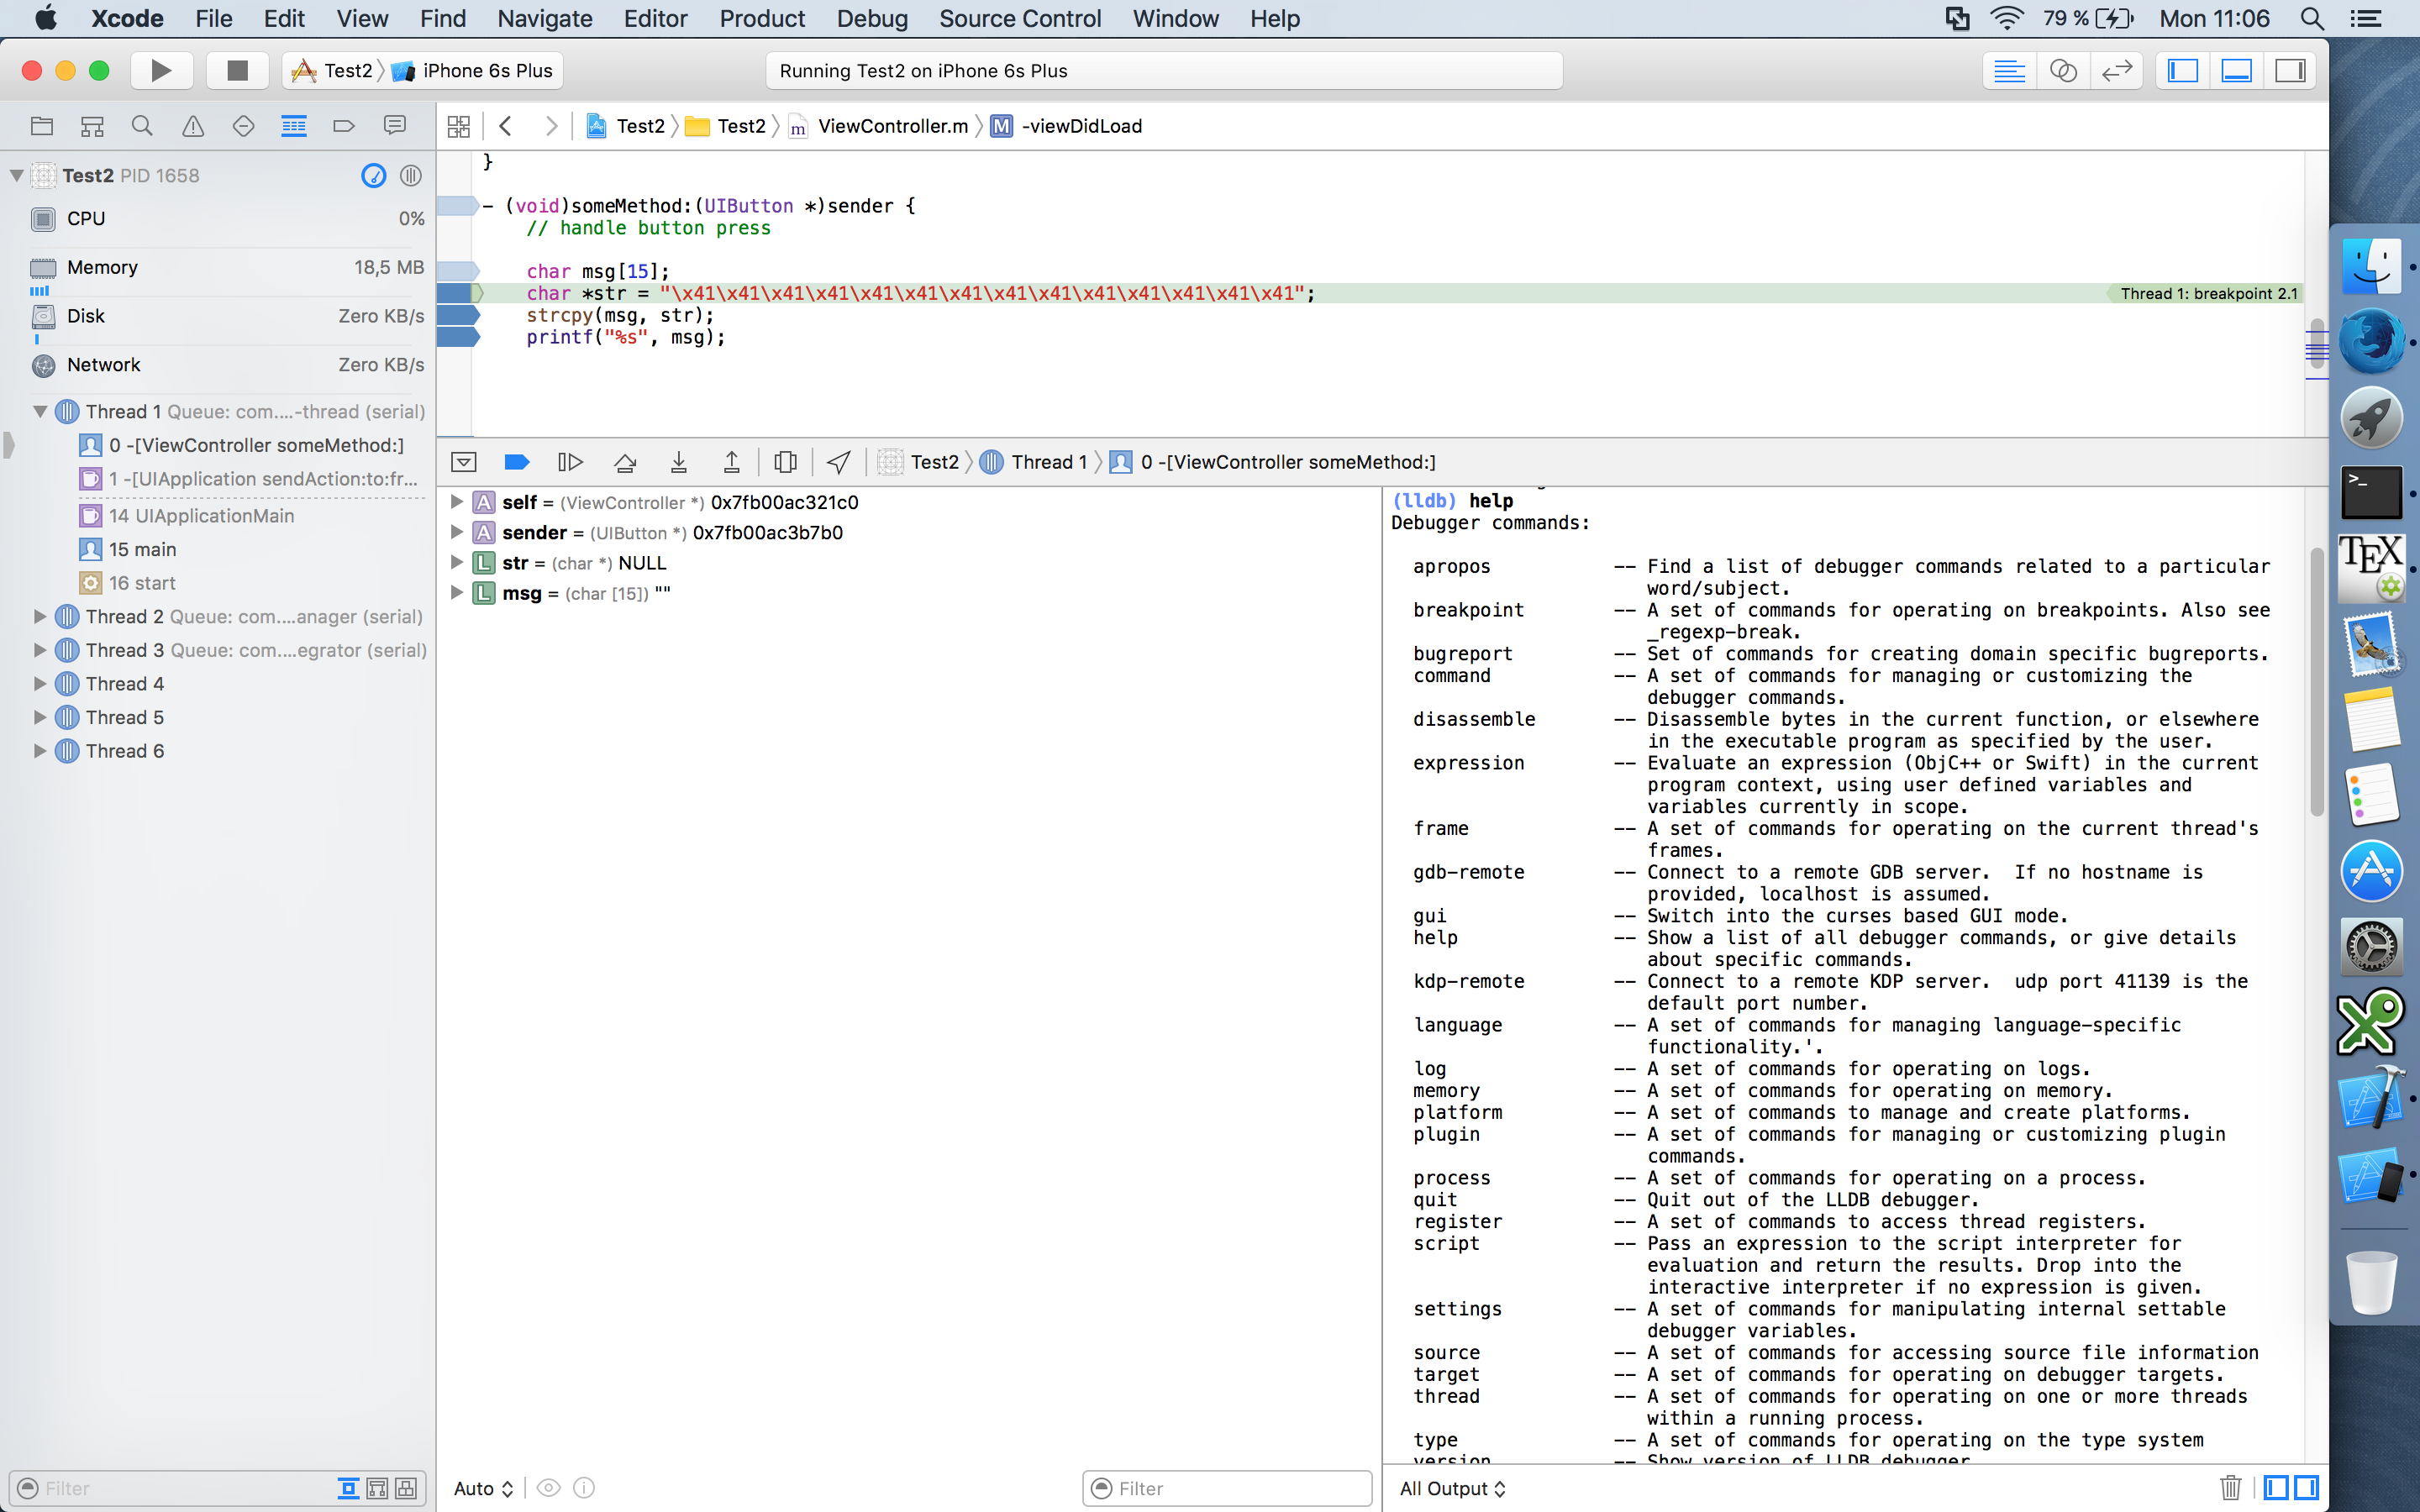
\includegraphics[width=\textwidth]{bilder/pentest_mobile_anwendungen/vergleich_aktuelle_situation/20160627_XCode-LLDB.png}
	\caption{LLDB in XCode}
	\label{fig:LLDBinXCode}
\end{figure}
Ein Ziel dieser Arbeit ist jedoch das Automatisieren von Analysen, weshalb das Ausführen der grafischen Oberfläche nicht optimal ist.

Leider ist nicht erkennbar, wie LLDB und das emulierte IPhone eine Verbindung herstellen. Eine Auflistung der offen Sockets auf dem System legt jedoch nahe, dass auf dem IPhone das Programm \textit{debugserver} gestartet wird, welches Remote-Debugging mit LLDB erlaubt. Es bleibt herauszufinden, wie die Debugging-Session auf dem simulierten IPhone ohne XCode hergestellt werden kann.

\begin{figure}[htbp]
	\centering
	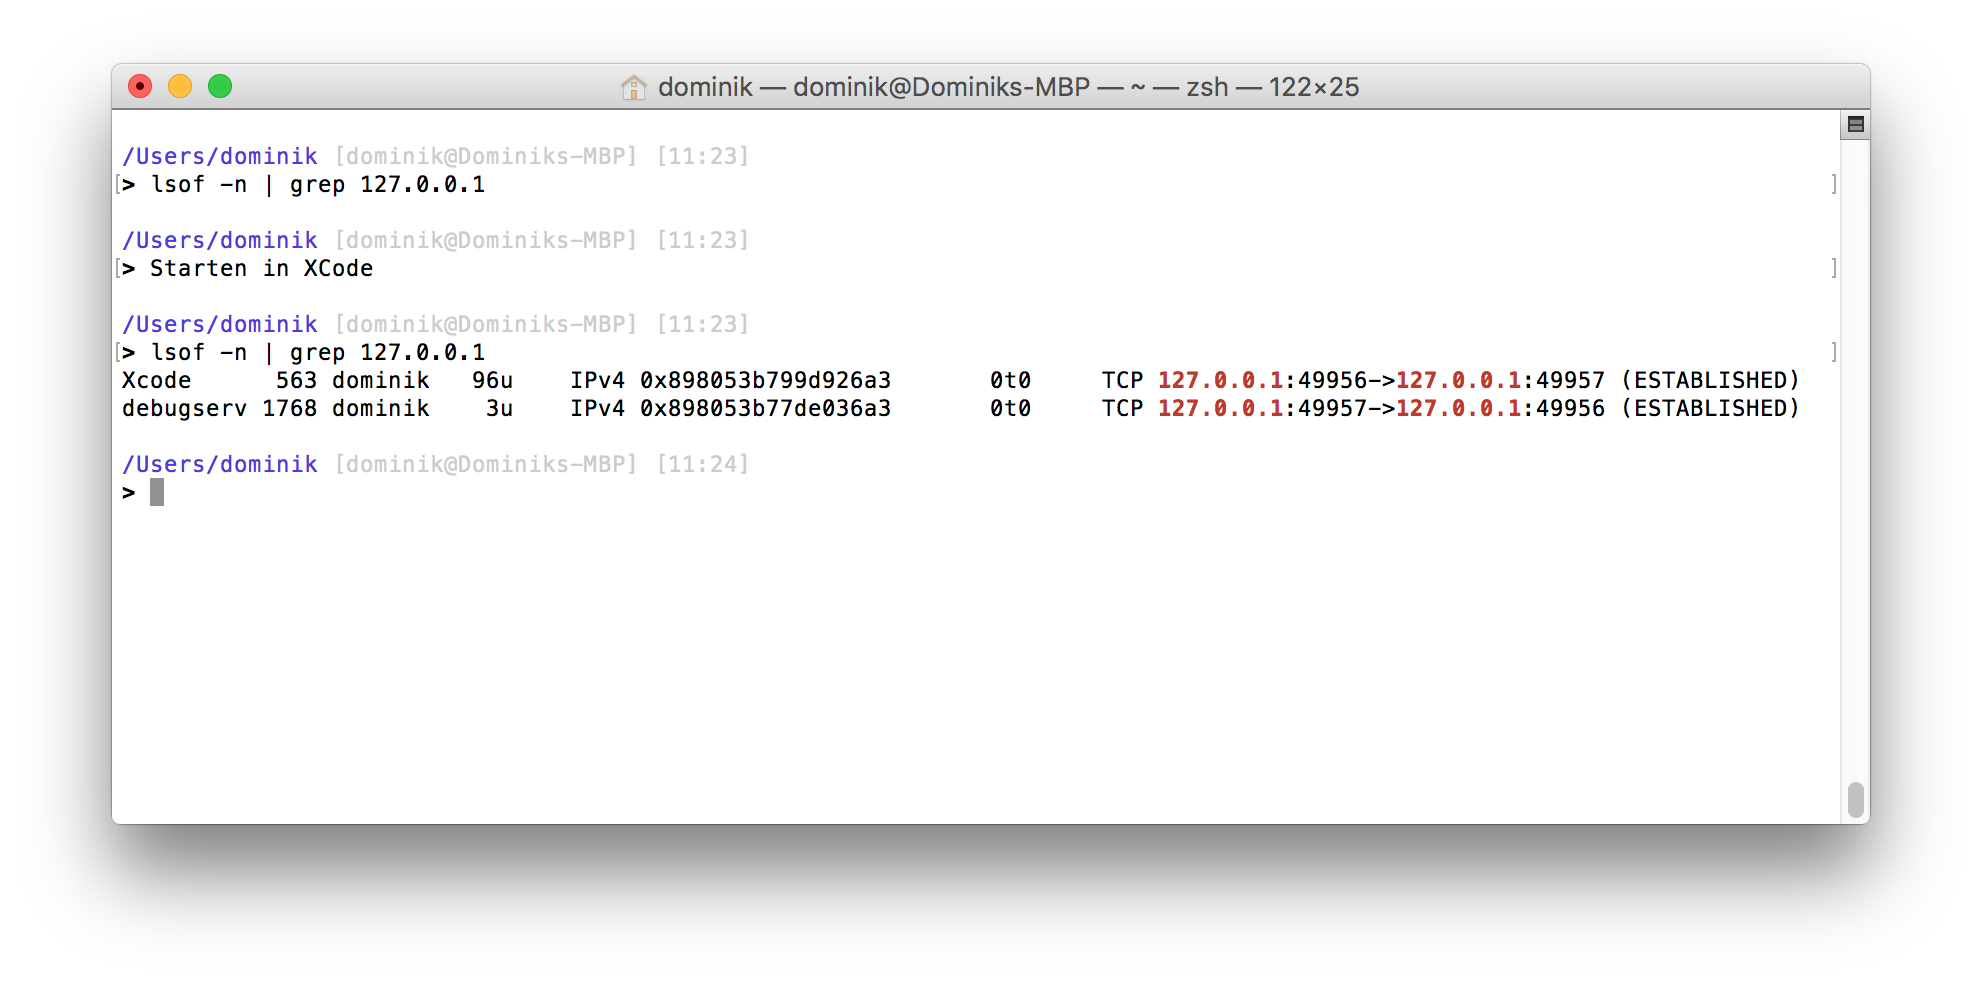
\includegraphics[width=\textwidth]{bilder/pentest_mobile_anwendungen/vergleich_aktuelle_situation/20160627_lsof_XCode_running.png}
	\caption{Vergleich der offenen Pipes vor und nach der Ausführung der Applikation in XCode}
	\label{fig:LSOFLLDB}
\end{figure}

Nach dem Artikel \url{https://developer.apple.com/library/ios/documentation/IDEs/Conceptual/gdb_to_lldb_transition_guide/document/lldb-terminal-workflow-tutorial.html} von Apple, ist es möglich, mit  LLDB eine App auch als "Standalone Debugger", also ohne XCode, zu verwenden. Dies ist in Abbildung \ref{fig:LLDBStandaloneDebugger} aufgezeigt.

\begin{figure}[htbp]
	\centering
	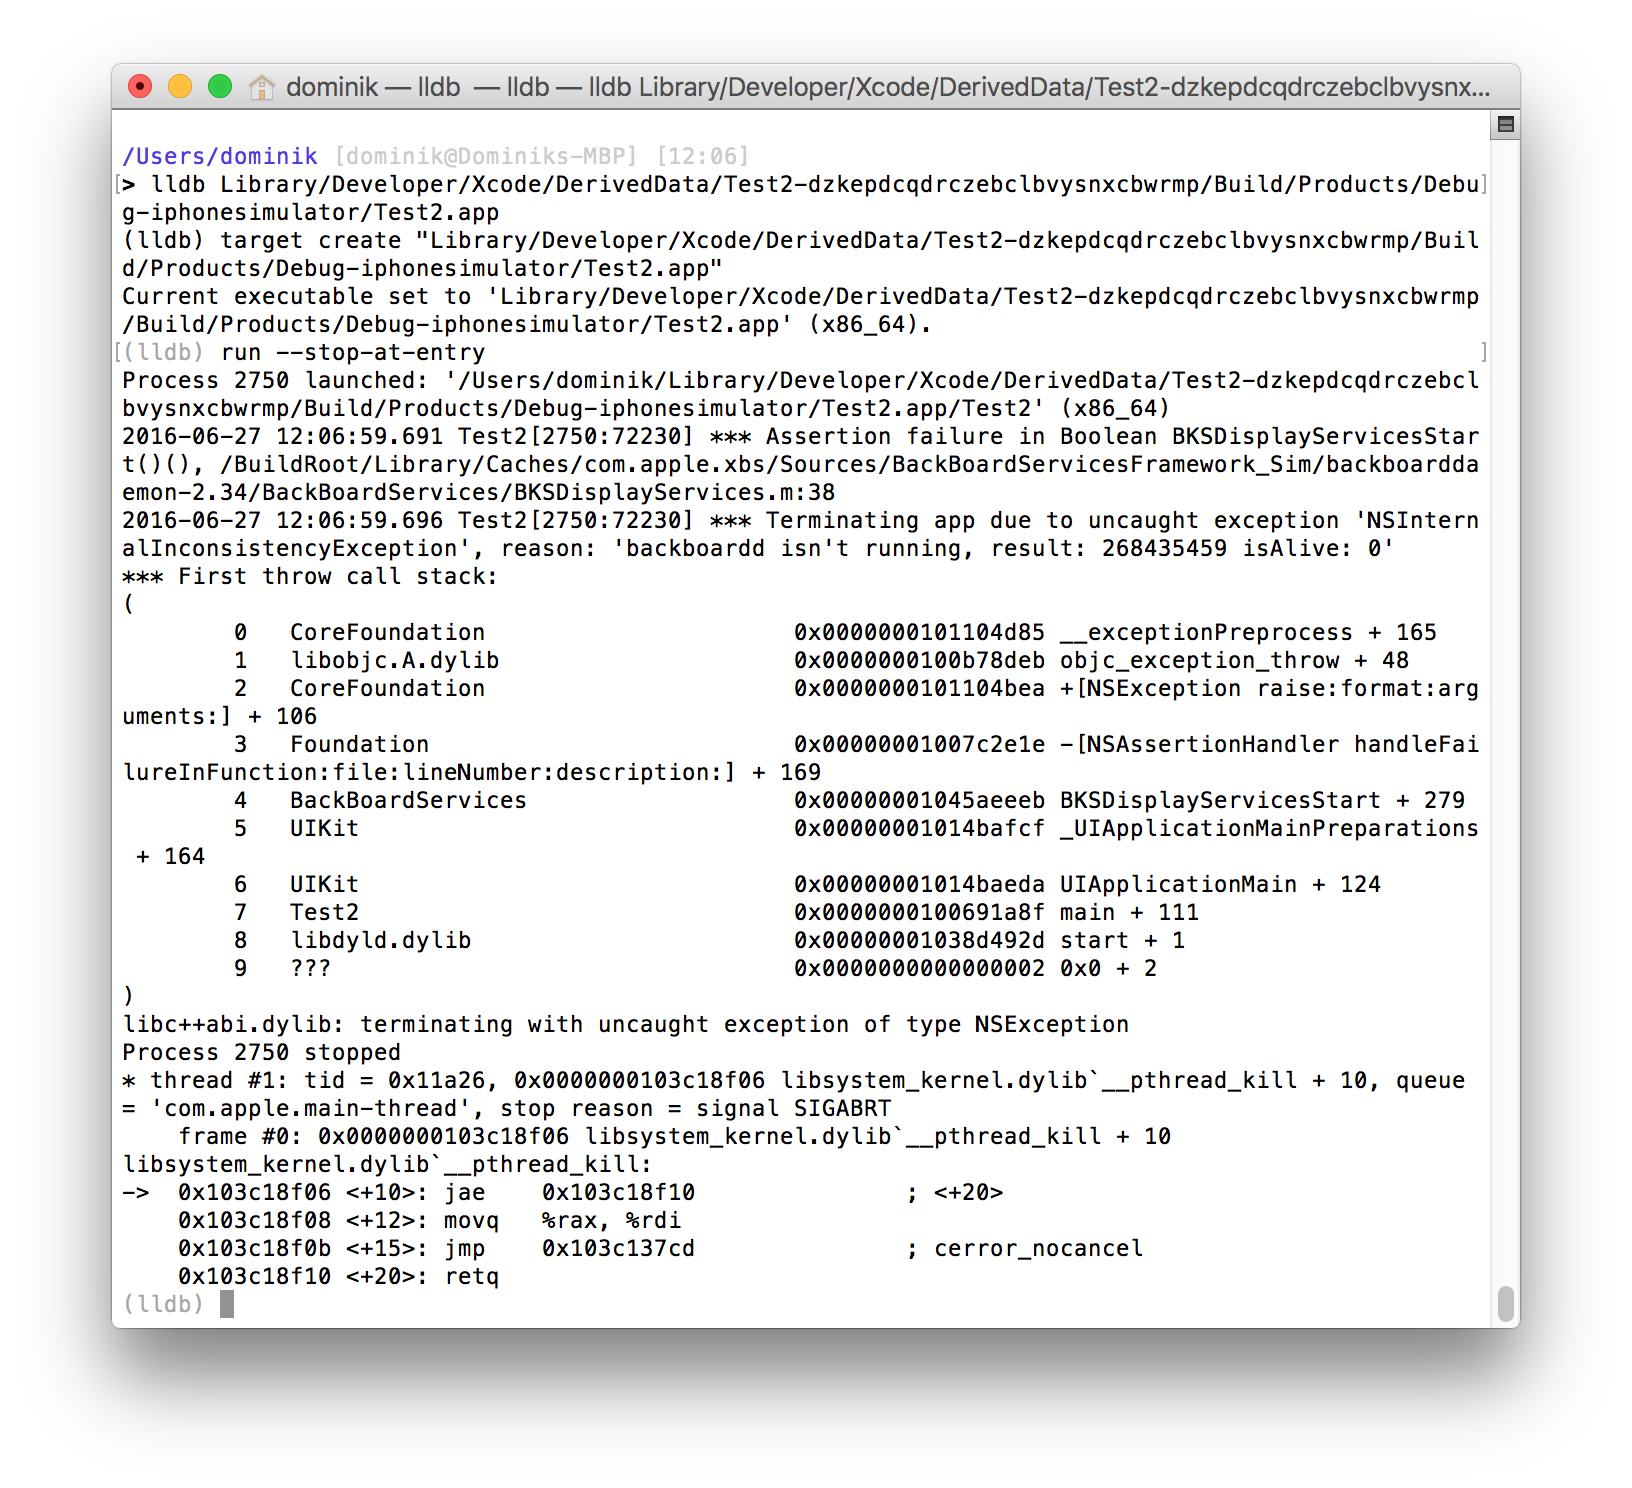
\includegraphics[width=\textwidth]{bilder/pentest_mobile_anwendungen/vergleich_aktuelle_situation/20160627_LLDB-Standalone-Debugger.png}
	\caption{LLDB als Standalone Debugger}
	\label{fig:LLDBStandaloneDebugger}
\end{figure}

Um zu verifizieren, dass die App auf einem simulierten IPhone ausgeführt wird, können entweder die geöffneten Prozesse (siehe Abbildung \ref{fig:LLDB-creating-IPhone-VM}) oder die geladenen Bibliotheken der Programme (siehe Abbildung \ref{fig:VergleichLLDBImages}) verglichen werden.

\begin{figure}[htbp]
	\centering
	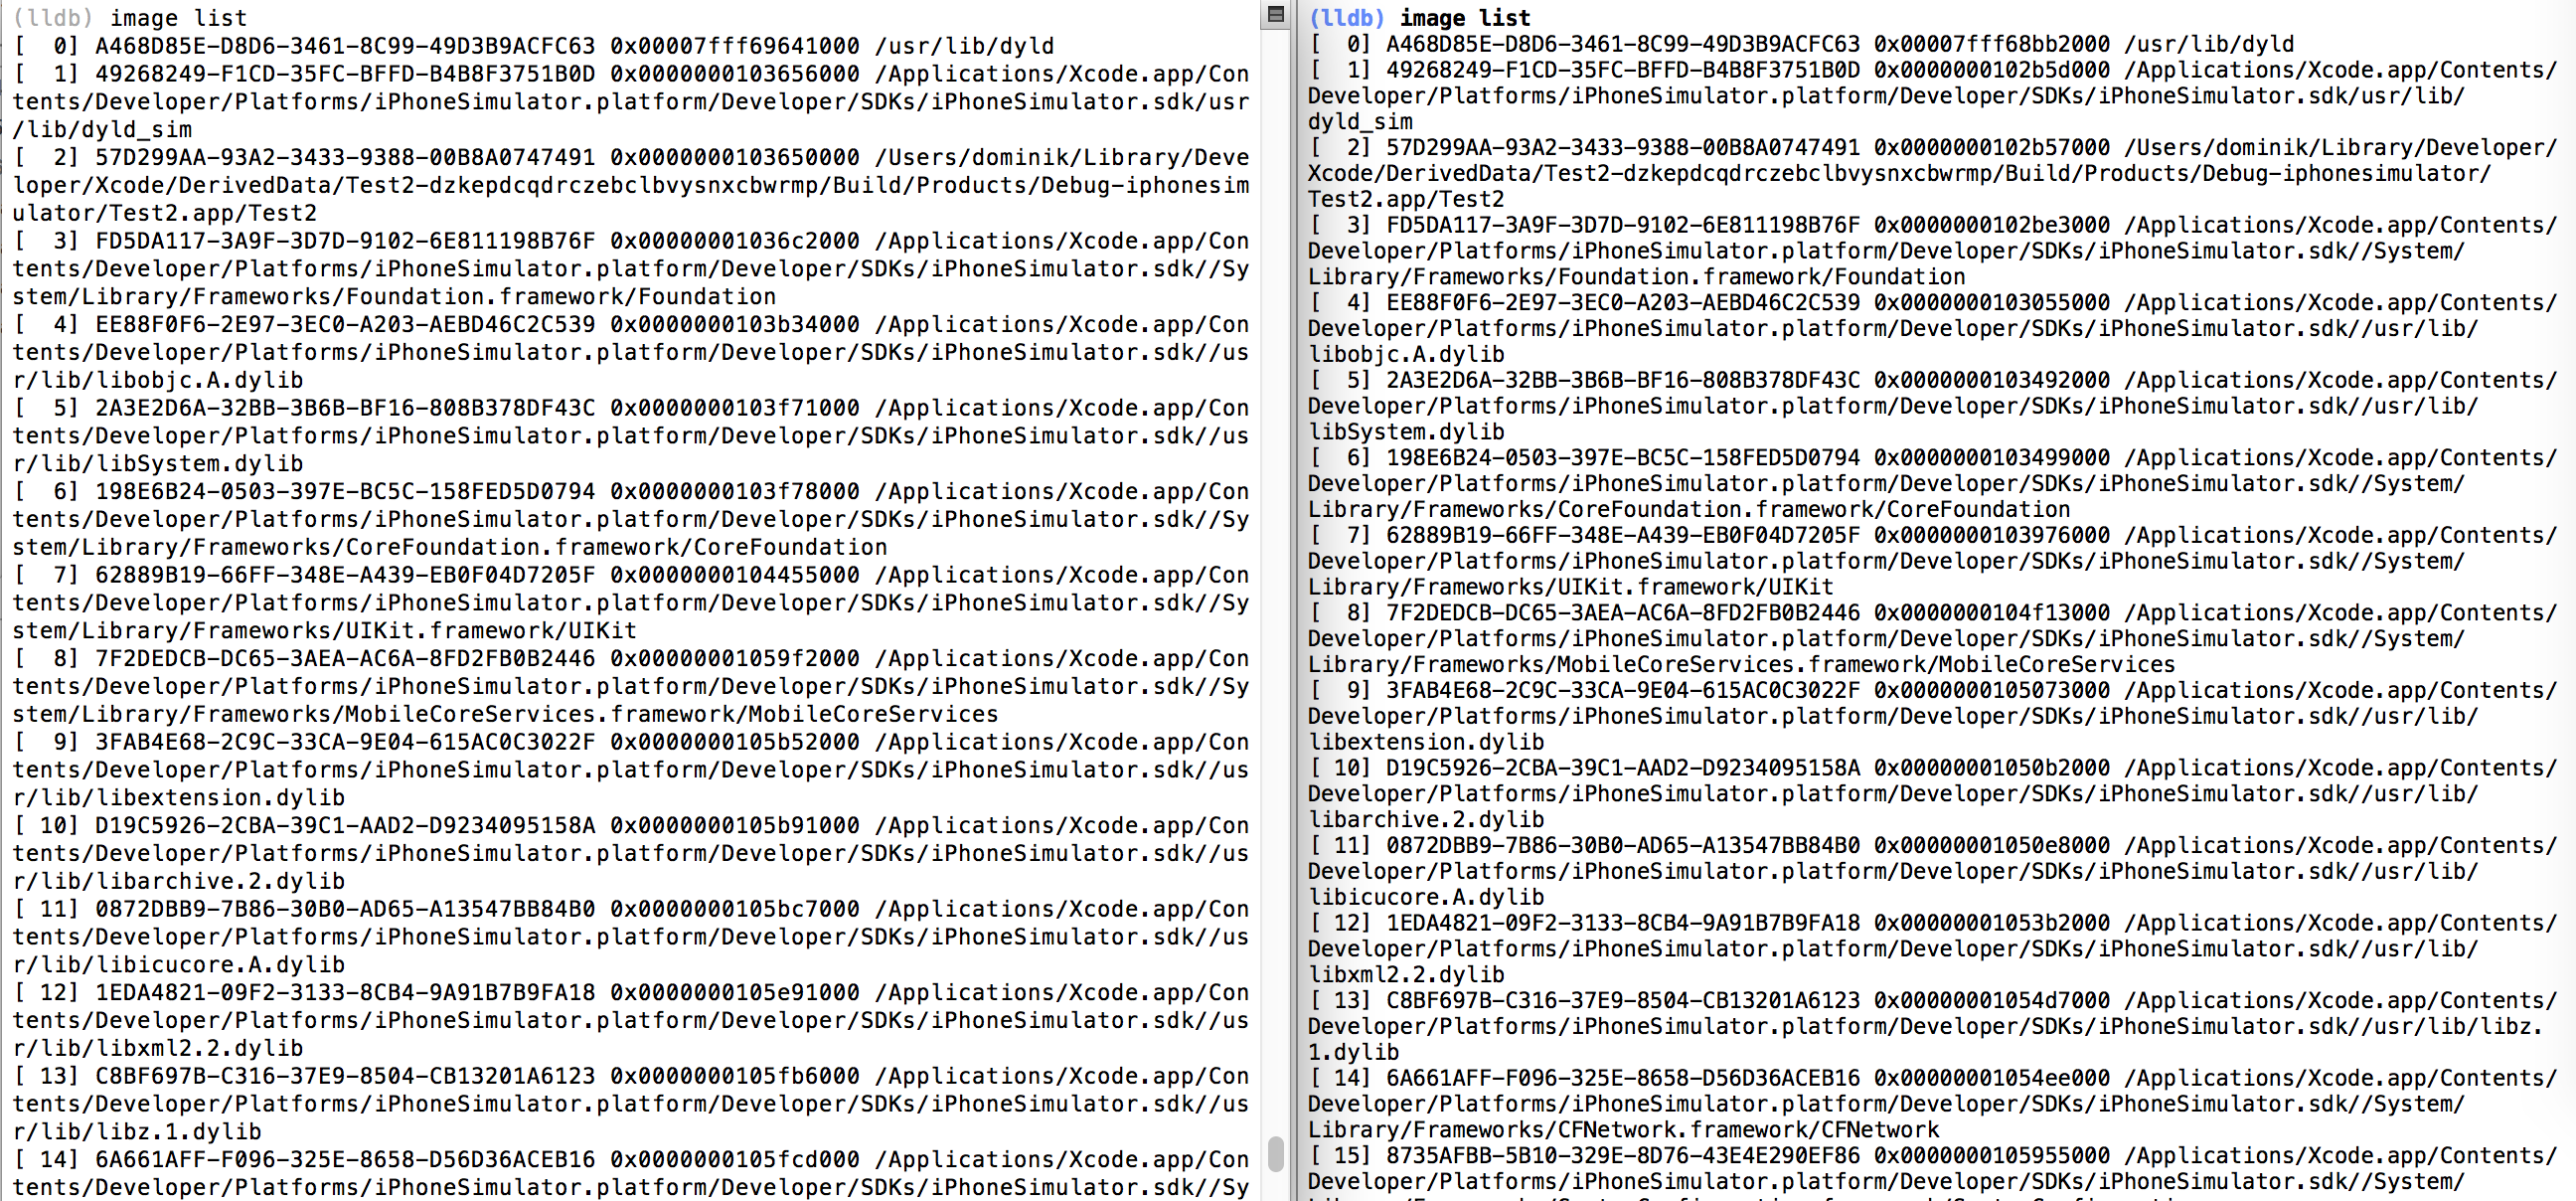
\includegraphics[width=\textwidth]{bilder/pentest_mobile_anwendungen/vergleich_aktuelle_situation/20160627_LLDB-image-list.png}
	\caption{LLDB als Standalone Debugger}
	\label{fig:VergleichLLDBImages}
\end{figure}

Bei Methoden zeigen, dass die App auf dem simulierten IPhone gestartet wird. Bei den Prozesse ist zu beobachten, dass vor Start von LLDB nur der Hintergrund-Service ausgeführt wurde. Nach dem Start von LLDB dagegen, läuft der gesamte Simulator.

Auch der Vergleich der geladenen Libaries legt nahe, dass die LLDB Standalone und XCode in der gleichen Umgebung ausgeführt werden. Die Adressen im RAM variieren aufgrund von ASLR zwar, aber es werden die Bibliotheken verwendet (am Pfad zu erkennen).

\begin{figure}[htbp]
\lstinputlisting[caption={Gestartete Prozesse nach LLDB Aufruf},lastline=16]{logs/20160627_LLDB-creating-IPhone-VM.txt}
\label{fig:LLDB-creating-IPhone-VM}
\end{figure}

\paragraph{Memory Corruption}
Bad Functions


\paragraph{Ungesicherte Verbindungen}$ $\\
https://developer.apple.com/library/ios/documentation/General/Reference/InfoPlistKeyReference/Articles/CocoaKeys.html unter NSAppTransportSecurity

\begin{lstlisting}
NSURL *url = [NSURL URLWithString:@"http://api.ipify.org"];
    NSData *data = [NSData dataWithContentsOfURL:url];
    NSString *ret = [[NSString alloc] initWithData:data encoding:NSUTF8StringEncoding];
    NSLog(@"ret=%@", ret);
\end{lstlisting}

\begin{lstlisting}
2016-06-28 08:42:56.518 Test2[4789:140270] App Transport Security has blocked a cleartext HTTP (http://) resource load since it is insecure. Temporary exceptions can be configured via your app's Info.plist file.
\end{lstlisting}


		\subsection{Windows-Phone}
			\subsubsection{Emulation vs. Hardware}
			VS
			\subsubsection{Debugging}
			VS	
		\subsection{Android}
			Android ist ein Ursprünglich 2003 von der Android, Inc. entwickeltes mobiles Betriebssystem. 2005 wurde es durch Google übernommen und wird seit dem weiterentwickelt. 2015 liegt es bei einem Marktanteil von TODO \%. Aufgrund der Quelloffenheit des Systems wird von vielen Herstellern auf verschiedensten Plattformen genutzt. Jedoch bringt die weitführende Fragmentierung des Betriebssystems auch Nachteile mit sich. So sind in 2015 nur TODO \% der Android-Devices auf einer aktuellen Version.\cite{Drake2014}
			\subsubsection{Android-Studio und SDK}
			Das Android-Studio ist eine umfassende IDE. Sie ermöglicht unter anderem das schnelle Entwickeln und Testen von Apps, sowie die Emulation von beliebigen Android-Versionen. Außerdem ist Android Studio kostenlos, Open-Source und für Linux, Mac und Windows erhältlich. Die aktuelle Version kann unter \url{http://developer.android.com/sdk/index.html} heruntergeladen werden. Die Installation unter Linux ist vergleichsweise einfach, da nur ein Archiv über das Kommando 
\begin{lstlisting}
unzip android-studio-ide-143.2739321-linux.zip
\end{lstlisting}
entpackt werden muss. Für alle anderen Betriebssysteme werden entsprechende Installationsroutinen zur Verfügung gestellt. Anschließend kann die IDE über die Datei "`bin/studio.sh"' gestartet werden. Neben dem Android-Studio gibt es noch das Android SDK, welches über die gleiche URL heruntergeladen werde kann. Es enthält wichtige Kommandozeilen-Tools wie \textit{adb}, \textit{fastboot} oder \textit{logcat}, auf welche im weiteren Verlauf noch detailliert eingegangen wird.
			\subsubsection{Compatibility Testing Suite}
			\cite{Drake2014} Seite 18
			\subsubsection{Emulation vs. Hardware}
			Android SDK
			\subsubsection{Debugging}	
			Android Debug Bridge\cite{androidDebugBridge}
			\subsubsection{Logcat}	
			Android Debug Bridge\cite{androidDebugBridge}	


	\section{Anforderungen und Abgleich mit MobSF}
	\begin{itemize}
		\item Automatisierung
		\item Blackbox/Whitebox
		\item Reporting
		\item False-Positive-Rate
	\end{itemize}

\section{Weiterentwicklung MobSF}
\label{Weiterentwicklung MobSF}
Ein Kernelement dieser Arbeit ist die Weiterentwicklung des Mobile Security Frameworks \textit{MobSF}. Die Funktionen des Frameworks sind bereits unter Abschnitt \ref{ref:PenMobAnwAbgAndMobSF} aufgezeigt. Im Folgenden sind die Änderungen dargestellt, welche an dem Framework vorgenommen und veröffentlicht wurden.

\subsection{Allgemeine Verbesserungen}
Neben Verbesserungen, welche einem genauen Bereich (\textit{Windows-Phone}, \textit{iOS}, \textit{Android}) zuzuordnen sind, gibt es auch einige allgemeine Erweiterungen am \textit{MobSF}. Diese sind im Folgenden dargestellt.

\subsubsection{Struktur}
Die Struktur von \textit{MobSF} war bisher relativ flach. Auf der ersten Ebene findet man die übergeordneten Module wie den \textit{ApiTester}, \textit{StaticAnalyzer}, \textit{DynamicAnalyzer} sowie den \textit{statischen Content}, \textit{Templates} und Kern-Module des \textit{MobSF}. Dies ist in der Abbildung \ref{fig:MobSFStrukOrig} verdeutlicht. Jedoch hatte die Struktur in den Modulen oft keine saubere Trennung der Aufgaben. So waren im \textit{StaticAnalyzer}-Modul sowohl \textit{iOS} wie auch \textit{Android}-Analyse in der \textit{views.py} zusammengefasst.\\

\begin{figure}[htbp]
\dirtree{%
.1 Mobile-Security-Framework-MobSF/.
    .2 .git/.
    .2 APITester/.
    .2 downloads/.
    .2 DynamicAnalyzer/.
    .2 LICENSES/.
    .2 logs/.
    .2 MalwareAnalyzer/.
    .2 MobSF/.
    .2 static/.
    .2 StaticAnalyzer/.
    .2 templates/.
    .2 uploads/.
}
\caption{Struktur des MobSF auf der ersten Ebene}
\label{fig:MobSFStrukOrig}
\end{figure}

\pagebreak
 Um hier eine klarere Trennung zu schaffen, wurde die \textit{views.py} in einem ersten Schritt aufgegliedert in drei Dateien:
\begin{description}
	\item[shared\_func.py: ] Die \textit{shared\_func.py} enthält alle Funktionen, welche sowohl für \textit{iOS} als auch \textit{Android} gebraucht werden. Beispiele sind die Erstellung von Hashes, das Generieren von PDFs oder das Entpacken von Archiven.
	
	\item[ios.py: ] Die Datei \textit{ios.py} enthält alle \textit{iOS} spezifischen Funktionen zur statischen Analyse.
	
	\item[android.py: ] Die Datei \textit{android.py} enthält alle \textit{Android} spezifischen Funktionen zur statischen Analyse.
	
	\item[windows.py: ] Die Datei \textit{windows.py} enthält alle \textit{Windows-Phone} spezifischen Funktionen zur statischen Analyse. Sie wurde nachträglich hinzugefügt (siehe \ref{Windows-Apps}), weshalb die Funktionen in der alten Struktur nicht auftauchen.
\end{description}
Dies ist im Detail in der Abbildung \ref{fig:MobSFStaticStrucVergl} dargestellt.\\

\begin{figure}
\centering
\begin{subfigure}{.5\textwidth}
  \dirtree{%
.1 StaticAnalyzer/.
    .2 [...].
    .2 views.py.
    	.3 key.
    	.3 PDF.
    	.3 Java.
    	.3 Smali.
    	.3 Find.
    	.3 ViewSource.
    	.3 ManifestView.
    	.3 StaticAnalyzer.
    	.3 GetHardcodedCertKeystore.
    	.3 ReadManifest.
    	.3 GetManifest.
    	.3 ValidAndroidZip.
    	.3 HashGen.
    	.3 FileSize.
    	.3 GenDownloads.
    	.3 zipdir.
    	.3 Unzip.
    	.3 FormatPermissions.
    	.3 CertInfo.
    	.3 WinFixJava.
    	.3 WinFixPython3.
    	.3 Dex2Jar.
    	.3 Dex2Smali.
    	.3 Jar2Java.
    	.3 Strings.
    	.3 ManifestData.
    	.3 ManifestAnalysis.
    	.3 CodeAnalysis.
    	.3 StaticAnalyzer\_iOS.
    	.3 ViewFile.
    	.3 readBinXML.
    	.3 HandleSqlite.
    	.3 iOS\_ListFiles.
    	.3 BinaryAnalysis.
    	.3 iOS\_Source\_Analysis.
}
  \caption{Alte Struktur}
  \label{fig:sub1}
\end{subfigure}%
\begin{subfigure}{.5\textwidth}
  \dirtree{%
.1 StaticAnalyzer/.
    .2 [...].
    .2 views/.
		.3 android.py.
	    	.4 [...].
	    	.4 GetHardcodedCertKeystore.
	    	.4 ReadManifest.
	    	.4 GetManifest.
	    	.4 ValidAndroidZip.
	    	.4 Dex2Jar.
	    	.4 Dex2Smali.
	    	.4 Jar2Java.
	    	.4 [...].
		.3 ios.py.
	    	.4 StaticAnalyzer\_iOS.
	    	.4 ViewFile.
	    	.4 readBinXML.
	    	.4 HandleSqlite.
	    	.4 iOS\_ListFiles.
	    	.4 BinaryAnalysis.
	    	.4 iOS\_Source\_Analysis.
	    .3 windows.py.
	    	.4 [...].
	    	.4 \_\_binskim.
	    	.4 \_\_binscope.
	    	.4 [...].
		.3 shared\_func.py.
	    	.4 key.
	    	.4 FileSize.
	    	.4 HashGen.
	    	.4 Unzip.
	    	.4 PDF.
}
  \caption{Neue Struktur}
  \label{fig:sub2}
\end{subfigure}
\caption{Vergleich der Struktur von \textit{StaticAnalyzer}}
\label{fig:MobSFStaticStrucVergl}
\end{figure}

Im weiteren Verlauf der Weiterentwicklung und mit der Einführung von Code-Standards (siehe \ref{pylintering}) wurde die Struktur weiter verfeinert. So wurden die Datei "`android.py"' entsprechend der Funktionalitäten weiter aufgeteilt. So ergibt sich für die statische Analyse von Android-Apps die in \ref{fig:MobSFStrukAndroid} dargestellte Dateistruktur.

\begin{figure}
\dirtree{%
.1 Mobile-Security-Framework-MobSF/.
	.2 [...].
    .2 StaticAnalyzer/.
    	.3 [...].
    	.3 views/.
            .4 \_\_init\_\_.py.
            .4 ios.py.
            .4 shared\_func.py.
            .4 windows.py.
            .4 android/.
                .5 \_\_init\_\_.py.
                .5 binary\_analysis.py.
                .5 cert\_analysis.py.
                .5 code\_analysis.py.
                .5 converter.py.
                .5 db\_interaction.py.
                .5 dvm\_permissions.py.
                .5 find.py.
                .5 java.py.
                .5 manifest\_analysis.py.
                .5 manifest\_view.py.
                .5 smali.py.
                .5 static\_analyzer.py.
                .5 strings.py.
                .5 view\_source.py.
                .5 win\_fixes.py.
}
\caption{Struktur der Dateien für die statische Analyse}
\label{fig:MobSFStrukAndroid}
\end{figure}

\newpage
\subsubsection{Code-Standards}\label{pylintering}
Um eine hohe Code-Qualität zu gewährleisten, sollte homogener und gut wartbarer Code geschrieben werden. Um dies über mehrere Entwickler hinweg zu gewährleisten, gibt es sogenannte \textit{Code-Standards}. Diese werden meist von einer zentralen Stelle festgelegt und beschreiben, zum Beispiel wie Variablen benannt werden müssen, wie viele Kommentare nötig sind und wie lang eine Funktion maximal sein darf.\\

Bei der Neu- oder Reimplementierung wurde auf die Verwendung von offiziellen \textit{Code-Standards} geachtet. Insbesondere wurde der\textit{ PEP 8} Standard \footnote{\url{https://www.python.org/dev/peps/pep-0008/}} für \textit{Python} verwendet, welcher die Lesbarkeit und Wartbarkeit von \textit{Python}-Code verbessern soll. Um die Einhaltung des Standards zu gewährleisten, wurde das Tool \textit{Pylint} verwendet. Dieses prüft einen gegebenen Quellcode gegen den Code-Standard \textit{PEP 8} und erzeugt entsprechende Warnungen für Abweichungen. Ursprünglich musste \textit{Pylint} auf der Konsole extra ausgeführt werden, jedoch können in moderne Entwicklungsumgebungen wie \textit{Atom} Tools wie \textit{Pylint} direkt eingebunden und genutzt werden. Dies hat den Vorteil, dass bereits während des Programmierens Verstöße gegen Standards oder Fehler wie zum Beispiel falsche Variablennamen entdeckt werden.\\

Für \textit{MobSF} wurde nicht von Anfang an mit Code-Standards entwickelt, weshalb zum Beispiel die Datei \textit{android.py} auf 2000 Code-Zeilen über 1600 \textit{Pylint}-Fehler aufwies. Durch aufwendige Refaktorierungs- und Umstrukturierungsarbeiten konnte die Anzahl der Abweichungen massiv reduziert werden.\\

Daraus ergibt sich erhöhte Wartbarkeit sowie eine einfachere Weiterentwicklung aufgrund weniger Merge-Konflikte. Dies ist möglich, da die jeweiligen Methoden je nach Funktionalität in entsprechende Module ausgelagert wurden und somit nur die eine, für die Funktion benötigte Datei, verändert und wieder in das Haupt-Projekt eingegliedert werden muss. Zuvor musste bei paralleler Entwicklung am Projekt jede auch noch so kleine Änderung in der übergreifenden Datei mit Änderungen einer parallel arbeitenden Partei zusammengeführt werden, was oftmals viel Arbeit bedeutet.

\subsubsection{strings}\label{ref:strings}
Zuerst wurde das \textit{MobSF} um die Fähigkeit erweitert, eine \textit{iOS}-Applikation mit dem \textit{strings}-Programm zu untersuchen. \textit{strings} durchsucht, sofern keine zusätzlichen Parameter übergeben werden, eine binäre Datei auf \textit{ASCII}-Elemente mit mindestens vier Stellen und gibt diese anschließend zurück.\\

Dies hilft oft bei einer ersten Einschätzung der Anwendung, da zumeist eine grundlegende Funktionsweise und der Zweck der Software abgeleitet werden können. Ebenso können eventuell unbeabsichtigt im Programm vergessene oder eigentlich geheime Strings in einer App aufgedeckt werden, wie zum Beispiel Entwicklerkommentare oder Passwörter. Auch sind je nach Compiler-Einstellungen Funktionsnamen oder Calls in andere Bereiche (z.B. Import-Table bei PE-Files) als String in einem Binary enthalten, was unter Abschnitt \ref{ref:WeitEntwWinBadFunc} zum Entdecken von verwundbaren Funktionen genutzt wird.\\

Sowohl \textit{Mac OS X} wie auch \textit{Linux} haben ein integriertes \textit{string}-Kommando, welches jedoch \textit{Windows} fehlt. Um die Multi-Platform-Fähigkeit weiterhin zu gewährleisten, wurde die Funktion in Python-Code abgebildet. Als Vorlage wurde ein bestehender Code von \textit{Stackoverflow} \footnote{\url{http://stackoverflow.com/a/17197027}} genutzt. Dieser lieferte jedoch eine wesentlich höhere Anzahl von Ergebnissen, da bestimmte Whitespace-Character ebenfalls beachtet wurden (siehe Abbildung \ref{lst:WeitMobSFVerglSrings}).\\

\begin{figure}[htbp]
\begin{lstlisting}
> wc -l strings_test_*
	  85149 strings_test_orig
  	541393 strings_test_pyth
    626542 total
\end{lstlisting}
\caption{Vergleich der gefundenen Strings mit Python und dem ursprünglichen Strings-Kommando}
\label{lst:WeitMobSFVerglSrings}
\end{figure}

Da viele der zusätzlich aufgedeckten Strings jedoch nicht bei der Analyse geholfen, sondern eher das Auffinden relevanter Strings erschwert haben, wurde der Originalcode wie in Abbildung \ref{lst:WeitMobSFStringsAnpassungen} dargestellt angepasst. Durch die Reduzierung der ausschlaggebenden Zeichen konnten die Ergebnisse optimiert werden, sodass eine effiziente Suche über Strings wieder möglich ist.

\begin{figure}[htbp]
\begin{lstlisting}[escapechar=\ü]
<<<<<<< Vor Anpassung
import string
=======
>>>>>>> Nach Anpassung

def strings(filename, min=4):
    """Print out all connected series of readable chars longer than min."""
    with open(filename, "rb") as f:
        result = ""
        for c in f.read():
<<<<<<< Vor Anpassung
            if c in string.printable:
=======
            if c in (
                    '0123456789'
                    'abcdefghijklmnopqrstuvwxyz'
                    'ABCDEFGHIJKLMNOPQRSTUVWXYZ'
                    '!ü"\#ü$%&\'()*+,-./:;<=>?@[\\]^_`{|}~ '
            ):
>>>>>>> Nach Anpassung
                result += c
                continue
            if len(result) >= min and result[0].isalnum():
                yield "'" + result + "'"
            result = ""
\end{lstlisting}
\caption{Anpassungen am Code der Python-Implementierung von Strings zur Verbesserung der Ergebnisse}
\label{lst:WeitMobSFStringsAnpassungen}
\end{figure}

\subsubsection{PDF-Generation}
Um eine effiziente Weitergabe der Ergebnisse zu ermöglichen, besitzt \textit{MobSF} eine PDF-Export-Funktion. Die Implementierung ist dabei relativ einfach. Es wird eine neue HTML-Sicht geschaffen, welche anschließend über das Python-Modul \textit{xhtml2pdf.pisa} als PDF geöffnet wird. Aufgrund von Leistungsproblemen des Moduls wurde später auf \textit{pdfkit}\footnote{\url{https://pypi.python.org/pypi/pdfkit}} gewechselt.\\

Eine solche Sicht wurde jeweils für alle Erweiterungen implementiert, welche in dieser Arbeit vorgenommen wurden.

\newpage
\subsubsection{RPC-Service}\label{ref:XMLRPC}
Um eine Kommunikation zwischen verschiedenen virtuellen Maschinen zu ermöglichen, wurde ein minimaler \textit{RPC-Server} in Python 3.5 entwickelt. Hierzu wurden verschiedene Ansätze untersucht. Getestet wurden hierzu die Python-Module \textit{Flask}, \textit{Requests}, \textit{xmlrpc} sowie \textit{RSA} zum Hinzufügen einer Authentisierung.

\paragraph{Flask}\label{ref:flask}
\textit{Flask} ist ein schneller, minimaler Webserver. Mit nur sehr wenig Code ist es möglich, eine Schnittstelle bereit zu stellen. Ein Code mit zwei akzeptierenden Funktionen, basierend auf der Schnellstart-Anleitung\footnote{\url{http://flask.pocoo.org/docs/0.10/quickstart/}}, ist in Abbildung \ref{ref:rpc_client.py} dargestellt.\\

\begin{figure}
\begin{lstlisting}
from flask import Flask
app = Flask(__name__)

@app.route('/')
def hello_world():
    print("Execute command!")
    return 'Hello World!'
    
@app.route('/second_command/')
def not_hello_world():
    print("Execute second command!")
    return 'Goodbye World!'

if __name__ == '__main__':
    app.run()
\end{lstlisting}
\caption{rpc\_client.py}
\label{ref:rpc_client.py}
\end{figure}

Es wird eine minimale Anwendung erstellt, welche auf dem Pfad "`\url{/}"' lokal das \textit{print}-Statement ausführt und den Text "`Hello World!"' zurück gibt. Wird die Anwendung unter dem Pfad "`\url{/second_command/}"' angesprochen, wird ein anderes \textit{print}-Statement ausgeführt und ein anderer Wert zurück gegeben. Auf diese Weise können schnell API-Funktionen auf verschiedene Pfade gelegt und angesprochen werden.

\newpage
\paragraph{Requests}
\textit{Requests} ist ein Python-Modul, welches einfache Anfragen (sogenannte \textit{Requests}) über HTTP(S) ermöglicht. So ist es über ein kurzes Code-Snippet, dargestellt in Abbildung \ref{ref:rpc_server.py}, möglich, die unter \ref{ref:rpc_client.py} aufgezeigt Schnittstelle anzusprechen.\\

\begin{figure}
\begin{lstlisting}
import requests

r = requests.get('http://localhost:5000')
print(r.text)

r = requests.get('http://localhost:5000/second_command/')
print(r.text)
\end{lstlisting}
\caption{rpc\_server.py}
\label{ref:rpc_server.py}
\end{figure}

Wird zuerst der Code \ref{ref:rpc_client.py} und anschließend der Code \ref{ref:rpc_server.py} ausgeführt, wird auf Server-Seite die in Abbildung \ref{lst:WeitMobSFRPCAusgClient} gezeigte Ausgabe erzeugt.\\
\begin{figure}[h]
\begin{lstlisting}
 $ python3 rpc_server.py
Hello World!
Goodbye World!
\end{lstlisting}
\caption{Ausgabe des RPC-Servers}
\label{lst:WeitMobSFRPCAusgServ}
\end{figure}

Auf der Client-Seite erfolgt die in Abbildung \ref{lst:WeitMobSFRPCAusgServ} dargestellte Ausgabe.
\begin{figure}[h]
\begin{lstlisting}
 $ python3 rpc_client.py
 * Running on http://127.0.0.1:5000/
Execute command!
127.0.0.1 - - [18/May/2016 19:10:56] "GET / HTTP/1.1" 200 -
Execute second command!
127.0.0.1 - - [18/May/2016 19:10:56] "GET /second_command/ HTTP/1.1" 200 -
\end{lstlisting}
\caption{Ausgabe des RPC-Clients}
\label{lst:WeitMobSFRPCAusgClient}
\end{figure}

Auf dieser Basis wurde die erste Version des RPC-Servers implementiert.

\newpage
\paragraph{xmlrpc mit rsa}
Bei der Eingliederung der Verbindung zwischen der virtuellen Maschine und dem Host wurde die Anforderung nach einer Möglichkeit zur Authentifizierung gefordert.\\

Zur Implementierung dieser Anforderung wurde das Python-Modul \textit{rsa} verwendet, welches sowohl für \textit{Python} 2 wie auch \textit{Python} 3 existiert. Die Ablauf der Kommunikation ist im Diagramm \ref{fig:WeitMobSFXMLRPCAblauf} dargestellt.\\

\tikzset{
    state/.style={
           rectangle,
           rounded corners,
           draw=black, very thick,
           minimum height=2em,
           inner sep=2pt,
           text centered,
           },
    bigbox/.style={
    		draw, 
    		inner sep=20pt,
    		label={[shift={(0ex,0ex)}]:#1}},
}

\begin{figure}[p]


\begin{tikzpicture}[node distance=4cm]

\node[state,initial]             (start) {Wartezustand};
\node[state,below=of start]             (an_start) {Analyse anfordern};
\node[state,right=of an_start]       (chal_calc) {Challenge berechnen};
\node[state,below =of an_start] (chal_sig) {Challenge signieren};
\node[state,below=of chal_calc] (check_chal) {Prüfen von Sig. und Chal.};
\node[state,below=of check_chal] (analyse) {Durchführung der Analyse};
\node[state,below=of chal_sig] (dar_erg) {Darstellung der Ergebnisse};

\node[bigbox=MobSF Host, label={[shift={(15ex,3ex)}]}, fit=(start)(an_start)(chal_sig)(dar_erg),] (MobSFHost) {};
\node[bigbox=Analyse Server, fit=(chal_calc)(check_chal)(analyse),] (MobSFHost) {};

\draw[-{Latex[width=3mm]}] (start) edge node [right]      {Analyse angefordert} (an_start);
\draw[-{Latex[width=3mm]}] (an_start) edge node [above]      {Challenge anfordern} (chal_calc);
\draw[-{Latex[width=3mm]}] (chal_calc) edge [out=260,in=90]node [above] {Challenge senden} (chal_sig);
\draw[-{Latex[width=3mm]}] (chal_sig) edge node [above] {Sig. Chal. senden} (check_chal);
\draw[-{Latex[width=3mm]}] (check_chal) edge node [left] {Analyse starten} (analyse);
\draw[-{Latex[width=3mm]}] (analyse) edge node [above=0.3cm] {Ergebnisse übertragen} (dar_erg);
\draw[-{Latex[width=3mm]}] (dar_erg) edge [out=125,in=235]node [left] {} (start);

\end{tikzpicture}
\caption{Ablauf einer Analyse auf einer separaten VM}
\label{fig:WeitMobSFXMLRPCAblauf}
\end{figure}

Durch das Signieren einer bei jedem Funktionsaufruf neu generierten Challenge ist sichergestellt, dass nur der echte Host die Funktion aufruft und keine \textit{Replay-Attacken} möglich sind.\\

Jedoch gab es bei der Implementierung über \textit{Flask} sowie mit den verschiedenen \textit{Python}-Versionen zwischen Server und Client Probleme beim Datenaustausch. So gibt es in \textit{Python} 2 einen dedizierten Variablen-Typ namens \textit{string}, wohingegen \textit{Python} 3 Strings in codierten Byte-Objekten speichert. Eine Konvertierung ist möglich und wurde umgesetzt. Jedoch legt \textit{Flask} eine weitere Ebene des Encodings über den übertragenen Inhalt, weshalb es leider nicht möglich war, die kryptographische Signatur fehlerfrei zu übertragen. Aus diesem Grund wurde nach weiteren und eventuell besser geeigneten Alternativen gesucht.\\

Nach einer kurzen Suche bot sich das Modul \textit{xmlrpclib} (\textit{Python} 2)/\textit{xmlrpc} (Python 3) an. Es ermöglicht die Kommunikation über das standardisierte XML-RPC-Protokoll\footnote{\url{http://xmlrpc.scripting.com/spec.html}} und ist somit unabhängig von der Python-Version. Zudem können Daten transparent zwischen Server und Client übergeben werden.

Es folgt ein kurzes Beispiel, in welcher ein Client eine \textit{hello\_world}-Funktion am Server aufruft. Dabei ist der Server-Code in Abbildung \ref{lst:WeitMobSFXMLRPCServerCode}, der Client Code in Abbildung \ref{lst:WeitMobSFXMLRPCClientCode} sowie die Ausgabe in Abbildung \ref{lst:WeitMobSFXMLRPCClientAusgabe} dargestellt.\\

\begin{figure}
\begin{lstlisting}
from xmlrpc.server import SimpleXMLRPCServer

def hello_world(name):
	"""Return an Hello-World for a name"""
    return "Hello World {}!".format(name)

if __name__ == '__main__':
	# Open the Server on port 8000
    server = SimpleXMLRPCServer(("0.0.0.0", 8000))
    server.register_function(hello_world, "hello_world")
\end{lstlisting}
\caption{XML-RPC Server Code}
\label{lst:WeitMobSFXMLRPCServerCode}
\end{figure}

\begin{figure}
\begin{lstlisting}
import xmlrpclib

proxy  = xmlrpclib.ServerProxy(
                "http://{}:{}".format(
                    TARGET_IP, 8000
                )
            )
print proxy.hello_world("John Doe")
\end{lstlisting}
\caption{XML-RPC Client Code}
\label{lst:WeitMobSFXMLRPCClientCode}
\end{figure}

\begin{figure}
\begin{lstlisting}
Hello World John Doe!
\end{lstlisting}
\caption{Ausgabe des Clients}
\label{lst:WeitMobSFXMLRPCClientAusgabe}
\end{figure}

Durch den minimalen Eingriff von \textit{xmlrpc} in die Kommunikation konnte die kryptographische Signatur als \textit{base64} codiertes Datum übergeben werden. Die Kern-Funktionen des Clients und Servers sind in den Abbildungen \ref{ref:WeitEntXMLClient} und \ref{ref:WeitEntXMLServer} dargestellt.\\

\begin{figure}
\begin{lstlisting}
def _get_token():
    """Get the authentication token for windows vm xmlrpc client."""
    challenge = proxy.get_challenge()
    priv_key = rsa.PrivateKey.load_pkcs1(
        open(settings.WINDOWS_VM_SECRET).read()
    )
    signature = rsa.sign(challenge, priv_key, 'SHA-512')
    sig_b64 = base64.b64encode(signature)
    return sig_b64
    
print proxy.test_challenge(_get_token())
\end{lstlisting}
\caption{Client-Code}
\label{ref:WeitEntXMLClient}
\end{figure}

\begin{figure}
\begin{lstlisting}
def _check_challenge(signature):
    signature = base64.b64decode(signature)
    try:
        rsa.verify(challenge.encode('utf-8'), signature, pub_key)
        print("[*] Challenge successfully verified.")
        _revoke_challenge()
    except rsa.pkcs1.VerificationError:
        print("[!] Received wrong signature for challenge.")
        raise Exception("Access Denied.")
    except (TypeError, AttributeError):
        print("[!] Challenge already unset.")
        raise Exception("Access Denied.")

def get_challenge():
    """Return an ascii challenge to validate authentication in _check_challenge."""
    global challenge
    # Not using os.urandom for Python 2/3 transfer errors
    challenge = ''.join(
        random.SystemRandom().choice(string.ascii_uppercase + string.digits) for _ in range(256)
    )
    return "{}".format(challenge)
    
def test_challenge(signature):
    """Test function to check if rsa is working."""
    _check_challenge(signature)
    print("Check complete")
    return "OK!"
\end{lstlisting}
\caption{Server-Code}
\label{ref:WeitEntXMLServer}
\end{figure}

Durch diese Art der Implementierung ist eine sichere, zuverlässige, effiziente und leicht erweiterbare Kommunikation zwischen Host und virtueller Maschine möglich.

\newpage
\subsection{Windows-Apps}
\label{Windows-Apps}
Seit Windows 8 und der damit eingeführten \textit{Unified Windows Platform}\footnote{\url{https://docs.microsoft.com/de-de/windows/uwp/get-started/universal-application-platform-guide}} sind moderne Windows-Apps unter Windows sowohl auf einem PC als auch auf einem Handy lauffähig.\\

Bisher hat das \textit{MobSF} noch keine Möglichkeit zur Prüfung von Windows-Apps bereitgestellt. Im Folgenden sind die im Rahmen dieser Arbeit implementierten Features beschrieben.

\subsubsection{Windows Phone Formats}
Um eine App analysieren zu können, muss zu allererst das File-Format betrachtet und verarbeitet werden. Leider sind im Windows-Umfeld diverse Formate gängig, von welchen im Folgenden einige in Hinblick auf Aufbau und Schutz analysiert werden.

\paragraph{XAP}
\textit{XAP} ist ein Format für \textit{Windows-Phone}-Apps ab \textit{Windows Phone 7} und enthält oft \textit{Silverlight}-Applikationen\footnote{\url{https://www.microsoft.com/silverlight/}}. Dementsprechend ist der Mime-Type zumeist \textit{application/x-silverlight-app}.\\

Ursprünglich war ein \textit{XAP}-File einfach ein \textit{ZIP}-Archiv, welches alle Dateien der App umfasst. Aus einem solchen \textit{XAP}-File konnte der Inhalt über folgende Schritte einfach gewonnen werden:
\begin{enumerate}
	\item \textit{XAP}-File herunterladen
	\item evtl. Dateiendung von "`.xap"' auf "`.zip"' ändern
	\item mit einem gängigen Archiv-Programm (z.B. 7-Zip) entpacken
\end{enumerate}
Anschließend liegen allen Dateien der App im Extraktion-Ordner.\\

\paragraph{APPX}
\textit{APPX} ersetzt ab Windows 8.1 das \textit{XAP}-Format. Auch das \textit{APPX}-Format nutzt einen Kompressionsalgorithmus ähnlich zu \textit{Zip}. Daher können Inhalte über das in Python integrierte Modul \textit{zipfile} extrahiert werden. Dies ist in Abbildung \ref{lst:WeitMobSFWinAPPXExtract} dargestellt.\\

\begin{figure}
\begin{lstlisting}
import zipfile
files=[]
with zipfile.ZipFile(APP_PATH, "r") as z:
        z.extractall(EXT_PATH)
        files=z.namelist()
return files
\end{lstlisting}
\caption{Beispiel-Code für das entpacken einer Windows-App}
\label{lst:WeitMobSFWinAPPXExtract}
\end{figure}

Es wurde folgende Mime-Types für \textit{APPX}-Dateien beobachtet:
\begin{itemize}
    \item \textit{application/octet-stream}
    \item \textit{application/vns.ms-appx}
    \item \textit{application/x-zip-compressed}
\end{itemize}

\paragraph{APPXBundle}
Das Format \textit{appxbundle} ist ein Zusammenschluss mehrerer \textit{APPX}-Dateien. Entsprechend ist der Mime-Type zum Beispiel \textit{application/zip} und kann ebenfalls mit zum Beispiel dem Python-Modul \textit{zipfile} oder einem gängigen Zip-Extraktions-Programm entpackt werden.

\paragraph{DRM}
Leider sind Apps aus dem Windows-Store häufig durch sogenanntes \textit{DRM} (\textit{Digital Rights Management}), hier \textit{Play Ready}, geschützt. Die Apps sind demnach nicht nur durch eine zertifikatsbasierte Signatur vor Veränderungen geschützt, sondern zusätzlich sind die App-Dateien mit \textit{AES} im \textit{CTR}-Mode verschlüsselt. Dies ist im \textit{PlayReady}-Header festgelegt, folgend ein Beispiel:
\begin{lstlisting}
<WRMHEADER xmlns="http://schemas.microsoft.com/DRM/2007/03/PlayReadyHeader" version="4.0.0.0">
  <DATA>
    <PROTECTINFO>
      <KEYLEN>16</KEYLEN>
      <ALGID>AESCTR</ALGID>
    </PROTECTINFO>
    <KID>5zhQkM1z5kq6HCCYD9nceQ==</KID>
    <LA_URL>http://microsoft.com/</LA_URL>
    <CUSTOMATTRIBUTES xmlns="">
      <S>rtXfkbbz4yuPNGrzjQc9yA==</S>
      <KGV>0</KGV>
    </CUSTOMATTRIBUTES>
    <CHECKSUM>TpkeZrwUjIY=</CHECKSUM>
  </DATA>
</WRMHEADER>
\end{lstlisting}

Zwar ist es möglich, \textit{DRM} geschützte Apps auf einem gerooteten Windows-Phone zu installieren und anschließend über Apps wie dem \textit{ProgramManager}\footnote{\url{https://forum.xda-developers.com/showthread.php?t=1922454}} als ungeschütztes Archiv an einen PC zu übertragen, jedoch könnte dies als Umgehung eines Kopierschutzes gesehen werden und wurde daher in dieser Arbeit nicht weiter verfolgt.

\newpage
\subsubsection{Virtuelle Maschine zur Analyse von Windows-Apps}
Da sowohl für die dynamische Analyse als auch aufgrund bestimmter Tools eine \textit{Windows}-VM notwendig ist, wird der Aufbau für \textit{MobSF} im Folgenden kurz allgemein dargestellt.\\

Als erstes muss ein Betriebssystem für die Analyse-VM gewählt werden. Der \textit{Windows-Phone}-Simulator steht ab \textit{Windows 8.1 64-Bit} zur Verfügung. Daher sollte \textit{Windows 8.1 64-Bit} oder höher verwendet werden. Hier wurde \textit{Windows 10 64-Bit} verwendet.\\

Für Tests bezüglich der dynamische Analyse wurde \textit{Visual Studio 2015} Community Edition verwendet. Da diese kostenlos ist, sind bis auf das Betriebssystem sind keine kostenpflichtigen Programme beteiligt.\\

Für die Kommunikation zwischen \textit{MobSF} und der VM wurde ein Setup-Skript (genauer beschrieben in Abschnitt \ref{ref:WeitMobSFWindSetup}) angefertigt, das die notwendigen Programme herunterlädt und die Installationen anstößt. Das Skript ist im Anhang unter \ref{ap:simcontrol} zu finden.

\subsubsection{Setup-Skript}\label{ref:WeitMobSFWindSetup}
Die Datei \textit{setup.py} wird über zwei verschiedene Wege aufgerufen, je nachdem ob \textit{MobSF} vollständig auf \textit{Windows} installiert wird oder nur die statische Analyse auf dem \textit{Windows}-System ausgeführt werden soll. Je nach Aufruf werden verschiedene Arbeitsschritte ausgeführt und auch verschiedene \textit{Python}-Versionen verwendet, weshalb manche Funktionen sowohl \textit{Python} 2- wie 3- kompatibel gestaltet sind. Dies führte im Rahmen dieser Arbeit zu einem erhöhten Implementierungsaufwand, jedoch muss kein Weiterentwicklungsaufwand betrieben werden, wenn der Kern von \textit{MobSF} ebenfalls auf \textit{Python} 3 portiert wird.

\paragraph{MobSF auf Windows}
Wird \textit{MobSF} vollständig auf \textit{Windows} installiert, wird das Setup-Script einmalig aus der \textit{settings.py} aufgerufen. Dabei wird \textit{Python} 2 verwendet. Anfangs wird das mit dem Download mitgelieferte Config-File in den richtigen Ordner des User-Kontext kopiert. Anschließend wird das Config-File über das ConfigParser-Modul geladen. Daraufhin werden alle notwendigen Ordner berechnet, in das Config-File geschrieben und angelegt. Damit sind die Vorbereitungen bezüglich der Config und der Ordner abgeschlossen.\\

Anschließend wird \textit{nuget} heruntergeladen. \textit{nuget} ist ein Paket-Manager für Windows, über welchen später \textit{BinSkim} installiert wird. Der Download ist in Python relativ einfach zu implementieren, wie in Listing \ref{lst:WeitNugetDown} dargestellt ist.\\

\begin{figure}
\begin{lstlisting}
# Open File
nuget_file_local = open(
	os.path.join(mobsf_subdir_tools, nuget_file_path), 
	"wb"
)

# Downloading File
print("[*] Downloading nuget..")
nuget_file = urlrequest.urlopen(nuget_url)

# Save content
print("[*] Saving to File {}".format(nuget_file_path))

# Write content to file
nuget_file_local.write(bytes(nuget_file.read()))

# Aaaand close
nuget_file_local.close()
\end{lstlisting}
\caption{Nuget-Download}
\label{lst:WeitNugetDown}
\end{figure}

Nachdem der Download abgeschlossen ist, wird \textit{BinSkim} über \textit{nuget} installiert. Dazu wird \textit{nuget} mit verschiedenen Parametern aufgerufen (siehe Listing \ref{lst:WeitNugetInst}).\\

\begin{figure}
\begin{lstlisting}
# Execute nuget to get binkim
output = subprocess.check_output(
    [
        nuget,
        "install", binskim_nuget, '-Pre',
        '-o', mobsf_subdir_tools
    ]
)
\end{lstlisting}
\caption{Installation von BinSkim über Nuget}
\label{lst:WeitNugetInst}
\end{figure}

Um später eine optimale Ausführung auf sowohl 64- wie 32-Bit Windows-System zu gewährleisten, werden aus den installierten Dateien die Binaries für \textit{BinSkim} \textit{x86} sowie \textit{x64} gesucht und in der Config-Datei gespeichert.\\

Als letztes Tool wird \textit{BinScope} installiert. Dies ist leider nicht über \textit{nuget} möglich. Daher muss eine \textit{MSI}-Datei heruntergeladen und anschließend installiert werden. Dabei muss der Installationspfad entsprechend gesetzt werden. Da dies nicht eindeutig von Microsoft dokumentiert ist, kann der Quellcode dem Appendix unter \ref{ap:BinScopeInstaller} entnommen werden.\\

Um sicherzustellen, dass das Setup-Script nicht mehrmals ausgeführt wird, wird zuletzt ein Lock-File platziert. Bei erneutem Start der Anwendung wird auf dieses geprüft und, falls es existiert, eine erneute Installation übersprungen.

\paragraph{Statische Analyse auf Windows}
Wird nur die statische Analyse auf \textit{Windows} durchgeführt, wird das Setup-Script direkt mit \textit{Python} 3 ausgeführt. Dabei wird ähnlich zur Installation auf Windows zuerst das Config-File initialisiert und anschließend werden die Ordner erstellt. Auch werden \textit{nuget}, \textit{BinSkim} und \textit{BinScope} installiert.\\

Die Ordnerstruktur wurde dabei anfangs wie folgt aufgebaut:

  \dirtree{%
.1 C:/.
    .2 [...].
    .2 MobSF/.
    	.3 Config/.
    		.4 config.txt.
    	.3 Download/.
    	.3 Tools/.    	
}

Um die Kompatibilität mit verschiedenen Systemkonfigurationen zu erhöhen, wurden später statt "`C"' die Ordner des Benutzers für die Speicherung der Programme verwendet.\\

Die \textit{config.txt} enthält Inhalte, welche zentral abgelegt werden und für verschiedene Skripte eine wichtige Rolle spielen. Ein Beispiel wäre der Pfad zum Verzeichnis, in welchem die Tools gespeichert werden. Der Download-Ordner enthält die durch das Setup-Skript heruntergeladenen Binaries, der Tools-Ordner die installierten Tools.\\

Zusätzlich zur lokalen Installation wird ein XMLRPC-Server unter Tools installiert und konfiguriert. Die genaue Funktionsweise dieses Services ist unter \ref{ref:XMLRPC} beschrieben.\\

Von Ajin Abraham, einem Contributor zu \textit{MobSF}, wurde nach der Implementierung ein ergänzendes Video zur Installation erstellt und auf Youtube veröffentlicht\footnote{\url{https://www.youtube.com/watch?v=17ilENuMj58}}.

\newpage
\subsubsection{Statische Analyse}
Um die drei marktführenden mobilen Betriebssysteme mit \textit{MobSF} abzudecken, wurden Funktionen für Windows-Phone-Apps hinzugefügt.\\

Zur statischen Analyse wurde das Tool \textit{binskim} von Microsoft getestet \footnote{\url{https://github.com/Microsoft/binskim/releases}}. Das Tool analysiert Compiler-Flags und verschiedenste andere statisch feststellbare Eigenschaften, bewertet diese und gibt die Ergebnisse im SARIF-Format\footnote{\url{https://github.com/sarif-standard/sarif-spec/}} zurück. Leider ist das Tool nur unter Windows ausführbar. Da \textit{MobSF} jedoch auch auf Linux und Mac OS X lauffähig sein soll, wird im Folgenden eine virtuelle Windows-Maschine zur statischen und dynamischen Analyse verwendet.

%\_CRT\_SECURE\_NO\_WARNINGS

\paragraph{Files}
Ein einfacher, aber oft sehr hilfreicher erster Eindruck entsteht durch die Auflistung der enthaltenen Files. In \textit{MobSF} existiert daher eine Methode, welche \textit{ZIP}-Archive entpackt und Pfad sowie Name der entpackten Dateien zurückliefert. Über diese Methode wurden auch hier die enthaltenen Files erfasst und in der Oberfläche dargestellt.

\paragraph{Bad Functions}\label{ref:WeitEntwWinBadFunc}
Ebenso wie bei \textit{iOS} wurde auch hier eine Extraktion der Strings aus dem Binary implementiert. Genutzt wurde dafür die unter \ref{ref:strings} entwickelte Implementierung des Strings-Kommandos in Python.\\

In diesen Strings sind ebenfalls die Namen der verwendeten Funktionen vorhanden, sodass jetzt auch hier eine Suche nach bekannterweise verwundbaren Funktionen implementiert wurde.

\newpage
\subsubsection{Zusätzlich eingebundene Tools zur statischen Analyse}\label{ref:WeitMobEingTools}
Im Folgenden werden die für die Analyse von Windows-Apps eingebundenen Tools vorgestellt.

\paragraph{BinSkim}
BinSkim ist ein Tool des \textit{Microsoft SDL} (\textit{Secure Development Lifecycle}) und prüft \textit{Windows}-Applikationen bezüglich der Konfiguration des Compilers/Linkers sowie andere Security-Relevante Merkmale.\cite{BinSkimGithub}\\

Dabei können folgende Fehlkonfigurationen erfasst werden:
\begin{description}
	\item[LoadImageAboveFourGigabyteAddress] 64-bit Images sollten eine \textit{base address} über der 4GB Grenze nutzen, um den Kompatibilitätsmodus von \textit{ASLR} nicht zu aktivieren. Dieser würde zu einem kleineren Raum für \textit{ASLR} und somit zu niedrigerer Sicherheit führen.
	
	\item[DoNotIncorporateVulnerableDependencies] Binaries sollten keine Abhängigkeiten zu Code mit bekannten Schwachstellen haben.
	
	\item[DoNotShipVulnerableBinaries] Es sollten keine Libraries enthalten sein, welche bekannte Schwachstellen besitzen.
	
	\item[BuildWithSecureTools] Applikationen sollten mit den aktuellsten Compiler- und Tool-Versionen kompiliert werden, um alle Sicherheitsfunktionen nutzen zu können.
	
	\item[EnableCriticalCompilerWarnings] Binaries sollten mit einem Warn-Level kompiliert werden, welcher alle Sicherheit-relevanten Checks angibt.
	
	\item[EnableControlFlowGuard] Binaries sollten das \textit{compiler control guard feature} (\textit{CFG}) zur BuildZeit aktivieren, um Angreifer davon abzuhalten, den Programmablauf zu verändern.
	
	\item[EnableAddressSpaceLayoutRandomization] Binaries sollten als \textit{DYNAMICBASE} gelinkt sein, um an \textit{ASLR} teilnehmen zu können.
	
	\item[DoNotMarkImportsSectionAsExecutable] PE-Import-Sektionen sollten nie gleichzeitig als schreibbar und ausführbar markiert sein.
	
	\item[EnableStackProtection] Binaries sollten \textit{stack protection} (zum Beispiel \textit{Stack-Canaries} über die \textit{/GS}-Flag) nutzen, um das Ausnutzen von \textit{stack buffer overflows} zu erschweren.
	
	\item[DoNotModifyStackProtectionCookie] Applikations-Code sollte keinen Einfluss auf die Stack-Absicherung haben.
	
	\item[InitializeStackProtection] Binaries sollten die Stack-Absicherung korrekt initialisieren, um das Ausnutzen von \textit{stack buffer overflows} zu erschweren.
	
	\item[DoNotDisableStackProtectionForFunctions] Applikations-Code sollte keine Stack-Absicherung für einzelne Funktionen abschalten.
	
	\item[EnableHighEntropyVirtualAddresses] Binaries sollten als kompatibel mit \textit{high entropy ASLR} markiert werden.
	
	\item[MarkImageAsNXCompatible] Binaries sollten das \textit{NX}-Bit gesetzt haben, um ungewollte Ausführung von Daten als Code zu verhindern.
	
	\item[EnableSafeSEH] X86 Binaries sollten \textit{SafeSEH} aktivieren, um das Ausnutzen von Memory-Schwachstellen zu erschweren.
	
	\item[DoNotMarkWritableSectionsAsShared] Code- und Data-Sections sollten nicht sowohl als \textit{shared} und \textit{writeable} markiert sein.
	
	\item[DoNotMarkWritableSectionsAsExecutable] PE-Sections sollten nicht sowohl \textit{writeable} wie auch \textit{executeable} sein.
	
	\item[SignSecurely] Images sollten über sichere kryptographische Signaturen vom einen vertrauenswürdigen Author geschützt sein.
\end{description}
$ $\\
Der originale Text sowie längere Beschreibungen sind dem Output des Kommandos
\begin{lstlisting}
BinSkim.exe exportRules output.json
\end{lstlisting}
zu entnehmen.

\paragraph{BinScope}
\textit{BinScope} ist ebenfalls ein Programm des \textit{Microsoft Secure Development Lifecycle} und untersucht ebenfalls Binaries auf fehlerhafte Konfigurationen. Es ist der Vorgänger zu \textit{BinSkim} und hat daher ähnliche Fehlerkategorien, welche im Folgenden dargestellt sind. Leider sind die Checks nicht dokumentiert, sodass der Autor aus den Namen und den bisher beobachteten Ergebnissen auf deren Funktionsweise schließt. \\

Im Gegensatz zu \textit{BinSkim} braucht \textit{BinScope} weniger Konfigurationsaufwand und ist daher, obwohl es der Vorgänger von \textit{BinSkim} ist, durchaus eine sinnvolle Ergänzung.

%\paragraph{Decompiler?}
%http://www.telerik.com/products/decompiler.aspx

\begin{description}
	\item[ATLVersionCheck] stellt sicher, dass die ATL-Header, welche für den Build des Binaries verwendet wurden, in Ordnung sind. Diese Regel kommt nur bei Dateien vom COM-Type zum Einsatz.
	
	\item[ATLVulnCheck] prüft, ob Klassen, welche IPersistStreamInit implementieren, potenziell verwundbare Eigenschaften aufweisen. Diese Regel kommt nur bei Dateien vom COM-Type zum Einsatz.
	
	\item[AppContainerCheck] prüft, ob die App mit der AppContainer-Flag kompiliert wurde. Die Flag ermöglicht eine isolierte Umgebung zur Ausführung der App\footnote{\url{https://msdn.microsoft.com/en-us/library/windows/desktop/mt595898(v=vs.85).aspx}}.
	
	\item[CompilerVersionCheck] prüft, ob für die App eine aktuelle Kompilerversion genutzt wurde (mindestens 14.00.50727).
	
	\item[DBCheck] prüft, ob das Binary mit der \textit{Dynamic Base}-Flag kompiliert wurde, also an \textit{ASLR} teilnehmen kann.
	
	\item[GSCheck] verifiziert, dass die \textit{/GS-Flag} beim Kompiliervorgang verwendet wurde, welche den \textit{Stack} vor \textit{Memory-Corruption} schützt (z.B. über \textit{Stack-Canaries}). 
	
	\item[DefaultGSCookieCheck] ist ein Check zur Konfiguration von GS, welcher die Art der verwendeten Cookies überprüft.
	
	\item[GSFriendlyInitCheck] ist ein Check zur Konfiguration von GS, welcher prüft, ob das Binary entsprechende GS-freundliche Einstiegspunkte bietet.
	
	\item[GSFunctionSafeBuffersCheck] ist ein weiterer Check zur Konfiguration von GS, welcher prüft, ob auch die Funktions-Buffer durch GS abgesichert werden.
	
	\item[ExecutableImportsCheck] prüft, ob die Import-Section als ausführbar markiert ist.
	
	\item[FunctionPointersCheck] prüft auf \textit{global function pointers}. Durch das Überschreiben von statischen Buffern können eventuell auch \textit{global function pointer} überschrieben werden, was eine Schwachstelle darstellen kann.

	\item[HighEntropyVACheck] prüft, ob für ASLR eine hohe Entropie zur Verfügung steht.
	
	\item[NXCheck] prüft, ob das NX-Flag (stehend für "`no execute"') gesetzt ist. Durch diese Maßnahme werden Exploits erschwert, da bestimme Speicherbereiche als nicht ausführbar gekennzeichnet werden.
	
	\item[RSA32Check] prüft auf 32-Bit RSA-Keys, für welche eine Primfaktorzerlegung leicht möglich wäre.
	
	\item[SafeSEHCheck] prüft, ob SafeSEH aktiviert wurde. Die Verwendung von SafeSEH verbessert das Fehlerhandling und erschwert die Entwicklung von Exploits.
	
	\item[SharedSectionCheck] prüft, ob Sections sowohl als \textit{shared} als auch \textit{writeable} markiert sind.
	
	\item[VB6Check] prüft, ob VB6-Code zum Einsatz kommt.
	
	\item[WXCheck] prüft, ob die WX-Flag verwendet wurde. Durch diese Flag müssen Linker-Warnungen wie Fehler behandelt werden, wodurch die Sicherheit erhöht wird.
\end{description}

\newpage
\subsection{iOS-Apps}
Ein weiteres wichtiges Betriebssystem ist das auf \textit{iPhones} verwendete \textit{iOS}.  Es hat einen Marktanteil von ca. $20\%$\cite{KatarWorldpanelMobBetrSys} und wird auch von Unternehmen immer häufiger genutzt. Umso wichtiger ist es, dass angebotene Apps entsprechend auf deren Sicherheit geprüft werden können. Daher sind im Folgenden durchgeführte Erweiterungen zu \textit{MobSF} aufgezeigt.

\subsubsection{IPA- und APP-Format}
Um eine \textit{iOS}-App zu analysieren, muss diese in einem passenden Format vorliegen. Geläufig und bereits von \textit{MobSF} unterstützt ist das \textit{IPA}-Format. Nativ werden \textit{iOS}-Apps jedoch als \textit{.app}-Dateien abgelegt. Die Umwandlung von \textit{.app} zu \textit{.ipa} ist über wenige manuelle Schritte zu verwirklichen. Kompiliert man eine App in \textit{Xcode}, wird diese unter einem bestimmten Pfad abgelegt. Der Standardpfad unter \textit{Xcode} 8 ist \textit{/Users/username/Library/Developer/Xcode/DerivedData/}. Alternativ kann der Pfad den Projekt-Einstellung in \textit{Xcode} über \textit{File $\rightarrow$ Projects Settings} entnommen werden. Die Struktur des \textit{DerivedData}-Ordner ist unter \ref{ref:deriveddata} dargestellt.\\

\begin{figure}
\dirtree{%
.1 DerivedData/.
    .2 \textit{Appname}-\textit{random}/.
    .2 \textit{Appname2}-\textit{random}/.
    	.3 Build/.
    		.4 Products/.
    			.5 \textit{Platform}/.
    				.6 \textit{Appname}.app.
    	.3 Index/.
    	.3 Logs/.
    	.3 TextIndex/.
    	.3 info.plist.
    	.3 scm.plist.    	
}
\caption{Struktur des DerivedData-Ordners}
\label{ref:deriveddata}
\end{figure}

Die \textit{.app}-Datei kann nun per Drag-n-Drop in den App-Bildschirm von \textit{iTunes} gezogen werden. Anschließend wird die App in \textit{iTunes} angelegt (siehe Grafik \ref{fig:itunes_app}). Wird die App per Drag-n-Drop wieder aus \textit{iTunes} in den Finder gezogen, wird die App als IPA-File abgelegt.

\begin{figure}[htbp]
	\centering
	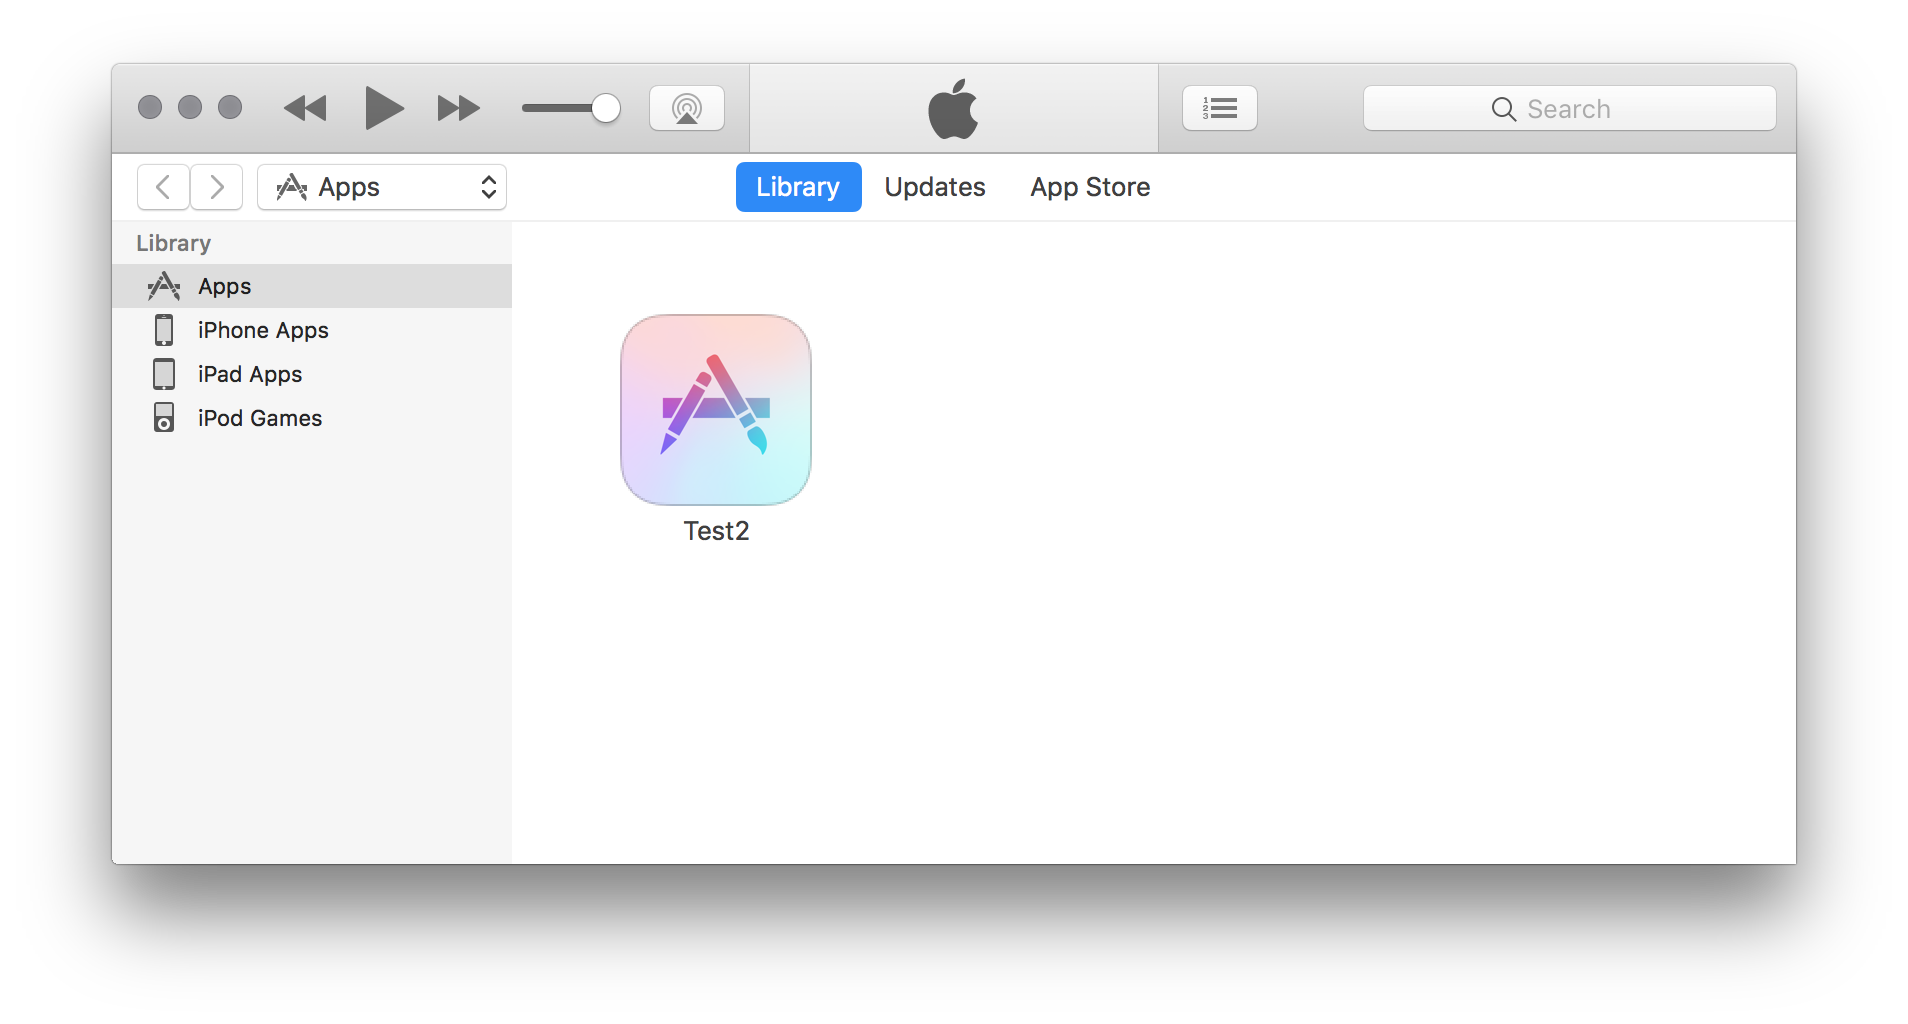
\includegraphics[width=\textwidth]{bilder/pentest_mobile_anwendungen/weiterentw_mobsf/itunes_app.png}
	\caption{iTunes-App-Fenster}
	\label{fig:itunes_app}
\end{figure}

\subsubsection{iOS-Permissions}
Eine wichtige Information über \textit{iOS}-Apps ist, welche Berechtigungen diese erfordern. In der aktuelle Version von \textit{iOS} müssen Berechtigungen, welche die App zur Laufzeit anfordert, in der \textit{info.plist} angekündigt werden. Im Folgenden sind die derzeit möglichen Berechtigungen aufgeführt.

\newpage
\begin{description}
	\item[NSAppleMusicUsageDescription]  beschreibt, dass die App den Zugriff auf die Musik-Bibliothek anfordern kann.
	
	\item[NSBluetoothPeripheralUsageDescription] beschreibt, dass die App die Berechtigung anfordern kann, auf das Bluetooth-Interface zuzugreifen.
	
	\item[NSCalendarsUsageDescription] beschreibt, dass die App den Zugriff auf den Kalender anfordern kann. Dadurch können alle Termine gelesen und verändert sowie gelöscht werden.
	
	\item[NSCameraUsageDescription] beschreibt, dass die App den Zugriff auf die Kamera anfordern kann. Dadurch können Fotos und Videos aufgenommen werden.
	
	\item[NSContactsUsageDescription] beschreibt, dass die App den Zugriff auf die Kontakte des User anfordern kann. Dadurch können alle Einträge im Kontaktbuch gelesen, verändert und gelöscht werden. 
	
	\item[NSHealthShareUsageDescription] beschreibt, dass die App den Lese-Zugriff auf die durch das Gerät erfassten Gesundheitsdaten anfordern kann. Diese können zum Beispiel zurückgelegte Strecken oder die Herzfrequenz enthalten.
	
	\item[NSHealthUpdateUsageDescription] beschreibt, dass die App den Schreib-Zugriff auf die Gesundheitsdaten des Users anfordern darf.
	
	\item[NSHomeKitUsageDescription] beschreibt, dass die App den Zugriff auf das Home-Kit des Users anfragen kann. Weitere Details zum Home-Kit sind auf der Apple-Webseite\footnote{\url{http://www.apple.com/de/ios/home/}} zu finden.
	
	\item[NSLocationAlwaysUsageDescription] beschreibt, dass die App das Recht anfragen kann, zu jeder Zeit den GPS-Standort des Users erfassen.
	
	\item[NSLocationWhenInUseUsageDescription] beschreibt, dass die App das Recht anfragen kann, den GPS-Standort auszulesen, solange die App im Vordergrund aktiv ist.
	
	\item[NSMicrophoneUsageDescription] beschreibt, dass die App das Recht anfragen kann, auf das Mikrophon zuzugreifen. 
	
	\item[NSMotionUsageDescription] beschreibt, dass die App den Zugriff auf den Motion-Sensor anfragen kann. Dadurch können Bewegungen erfasst werden.
	
	\item[NSPhotoLibraryUsageDescription] beschreibt, dass die App den Zugriff auf die Photo-Bibliothek anfordern kann.
	
	\item[NSRemindersUsageDescription] beschreibt, dass die App den Zugriff auf die Reminder des Users anfordern kann. Dadurch können Reminder ausgelesen, erstellt, verändert oder gelöscht werden.
	
	\item[NSVideoSubscriberAccountUsageDescription] beschreibt, dass die App den Zugriff auf den TV-Account des Users anfragen kann.
\end{description}

Diese, sowie weitere Einträge für die \textit{Info.plist} sind der Apple-Dokumentation zu entnehmen \footnote{\url{https://developer.apple.com/library/content/documentation/General/Reference/InfoPlistKeyReference/Articles/CocoaKeys.html}}.\\

In der Auflistung wurde die Formulierung "`anfragen kann"' genutzt, da der Eintrag in der \textit{info.plist} der App nicht automatisch die Rechte gibt, sondern der User diese bestätigen muss, sobald die App diese wirklich anfordert. Jedoch können zur Laufzeit keine Rechte angefordert werden, welche nicht vorher in der \textit{info.plist} festgelegt wurden.\\

Um in \textit{MobSF} die Berechtigungen auszulesen, wurde dementsprechend die \textit{info.plist} ausgelesen und auf die entsprechenden Einträge geprüft. Da die Datei jedoch im Binärformat vorliegt, muss diese zuerst umgewandelt werden. Dies kann über das in \textit{Xcode} enthaltene Tool \textit{plutil} erreicht werden. Der Aufruf ist dabei wie folgt:
\begin{lstlisting}
plutil -convert xml1 info.plist
\end{lstlisting}
Anschließend kann über das in Python enthaltene Modul \textit{plistlib} wie folgt auf die Einträge zugegriffen werden:
\begin{lstlisting}
p_list = plistlib.readPlistFromString(read_bin_xml(converted_info_plist_file))
if "NSBluetoothPeripheralUsageDescription" in p_list:
        print("Bluetooth-Permission found!")
\end{lstlisting}

\pagebreak
In \textit{MobSF} wird auf diese Art die \textit{info.plist}-Datei verarbeitet und die Ergebnisse in der Web-Oberfläche dargestellt. Das Ergebnis für eine App mit Bluetooth-Berechtigung ist in Grafik \ref{fig:permission_check} dargestellt.\\

Auf einige Rechte wie den Zugriff auf Kontakte, Kalender, Reminder, Kamera und Mikrophon sollte bei Analyse besonders geachtet werden.

\subsubsection{Erkennung von ungesicherten Verbindungen}\label{ref:WeitMobSFErkennungVonUngesichertenVerbindungen}
Wie in \ref{ref:inseccon} unter "`Ungesicherte Verbindungen"' beschrieben, müssen ab \textit{iOS} 9.0 Apps den  RFC-Standard 2818\footnote{\url{https://tools.ietf.org/html/rfc2818}} nutzen, um Verbindungen zu Webseiten oder APIs aufzubauen.\\

Daher wurde \textit{MobSF} um ein Feature ergänzt, welches die \textit{Info.plist} auf Ausnahmen überprüft. Der Code ist unter Abbildung \ref{lis:NSAppTransportSecurity} dargestellt.\\

\begin{figure}
	\begin{lstlisting}
def __check_insecure_connections(p_list):
    '''Check info.plist for insecure connection configurations.'''
    print "[INFO] Checking for Insecure Connections"

    insecure_connections = []

    if 'NSAppTransportSecurity' in p_list:
        ns_app_trans_dic = p_list['NSAppTransportSecurity']
        if 'NSExceptionDomains' in ns_app_trans_dic:
            for key in ns_app_trans_dic['NSExceptionDomains']:
                insecure_connections.append(key)

    return insecure_connections
	\end{lstlisting}
	\caption{Auslesen von Ausnahmen bezüglich der TLS-Konfiguration aus der Info.plist}
	\label{lis:NSAppTransportSecurity}
\end{figure}

\begin{figure}[htbp]
	\centering
	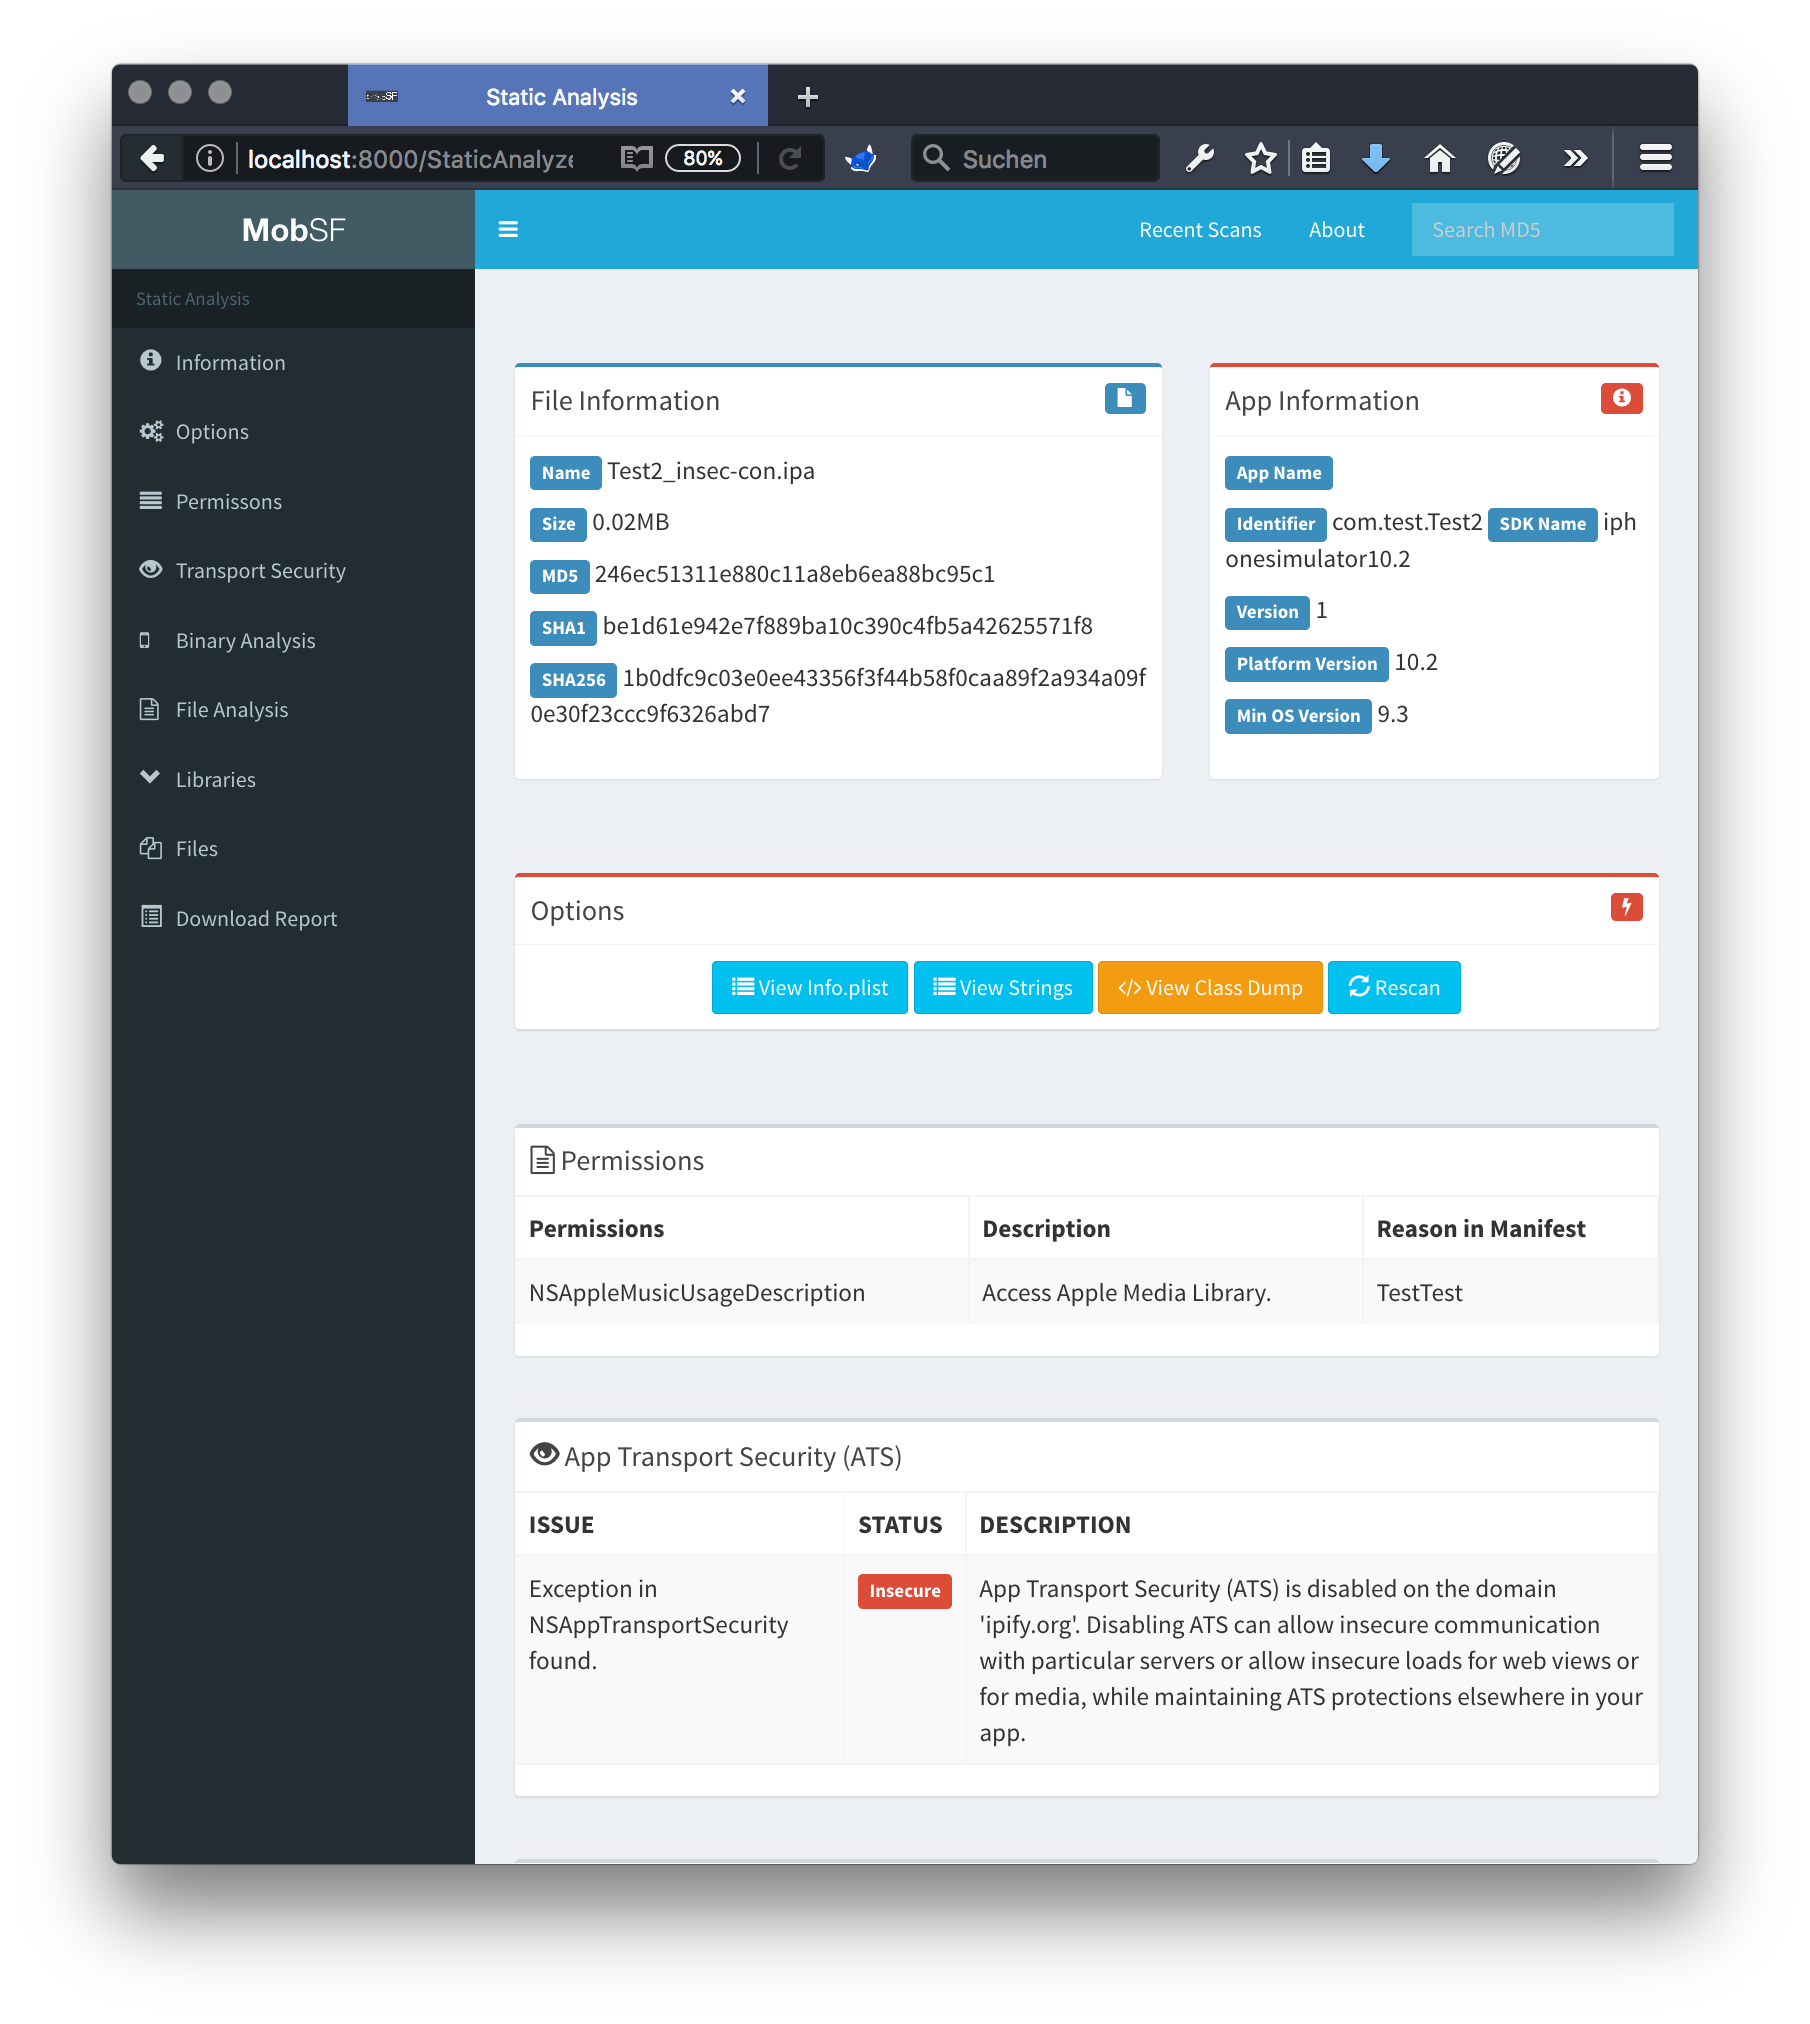
\includegraphics[width=\textwidth]{bilder/pentest_mobile_anwendungen/weiterentw_mobsf/perm_con_check.png}
	\caption{Ergebnis für eine App mit Bluetooth-Berechtigung und einer Ausnahme der \textit{ATS}}
	\label{fig:permission_check}
\end{figure}


Werden Ausnahmen gefunden, werden diese in der HTML-Oberfläche dargestellt. Ein Beispiel ist in \ref{fig:permission_check} zu sehen.


\subsubsection{Dynamische Analyse über Simulator}
Im Rahmen dieser Masterarbeit wurden ebenfalls Möglichkeiten getestet, wie eine dynamische Analyse von \textit{iOS}-Apps über den "`Simulator"' abgebildet werden könnte. Um dieses Ziel zu erreichen, muss zuerst eine Automatisierung des Simulators möglich sein. Diese Automatisierung kann über das in \textit{Xcode} enthaltene Tool "`xcrun"' realisiert werden.\\

%Einige für die Automatisierung relevante Parameter sind im Folgenden aufgeführt.
%\begin{description}
%	\item[boot] startet ein bereits existierendes virtuelles Gerät.
%	\item[shutdown] fährt ein gestartetes herunter.
%	\item[delete] löscht ein Gerät.
%	\item[openurl] öffnet eine URL auf einem gestarteten Gerät.
%	\item[install] installiert eine App anhand einer \textit{.app} auf einem Gerät.
%	\item[uninstall] deinstalliert eine App vom Gerät.
%	\item[launch] öffnet eine bereits installierte App auf einem Gerät.
%	\item[terminate] beendet eine bereits gestartete App auf einem Gerät.
%\end{description}

\pagebreak
Über die Befehle von \textit{xcrun} kann folgender Ablauf für die dynamische Analyse realisiert werden.
\begin{enumerate}
	\item Gerät starten (Parameter \textit{boot})
	\item App installieren (Parameter \textit{install})
	\item App ausführen (Parameter \textit{launch})
	\item Analyse durchführen
	\item App schließen (Parameter \textit{termiate})
	\item App deinstallieren (Parameter \textit{uninstall})
	\item Gerät herunterfahren/ggf. löschen (Parameter \textit{shutdown} oder \textit{delete})
\end{enumerate}
Somit sollte für erste Tests ein geeigneter Ablauf zur Verfügung stehen. Alternativ hätte ein Tool von \textit{Facebook}\footnote{\url{https://github.com/facebook/FBSimulatorControl}} genutzt werden können, welches wohl einen ähnlichen Funktionsumfang besitzt. Da das Ziel jedoch eine Eingliederung in MobSF war, wurde die Eigenimplementierung über \textit{xcrun} gewählt.\\

Ein Kerninhalt der dynamischen Analyse ist zumeist der Netzwerkverkehr. Eine simple Aufzeichnung über \textit{TCPDump} oder \textit{Wireshark} kann natürlich leicht vollzogen werden. Um dies jedoch zu verifizieren, wurde eine App mit dem in Abbildung \ref{lis:WeitMobSFiOSOpenURLSec} gezeigten Code angelegt.\\

\begin{figure}[htbp]
\begin{lstlisting}
NSURL *url = [NSURL URLWithString:@"https://api.ipify.org"];
SData *data = [NSData dataWithContentsOfURL:url];
NSString *ret = [[NSString alloc] initWithData:data encoding:NSUTF8StringEncoding];
\end{lstlisting}
\caption{Aufruf von \url{https://api.apify.org}}
\label{lis:WeitMobSFiOSOpenURLSec}
\end{figure}

Die \textit{Wireshark}-Ausgabe verifiziert, dass die Verbindung aufgezeichnet werden kann, wie in Grafik \ref{fig:WeitMobSFiOSWireshark} zu sehen ist.\\

\begin{figure}[htbp]
	\centering
	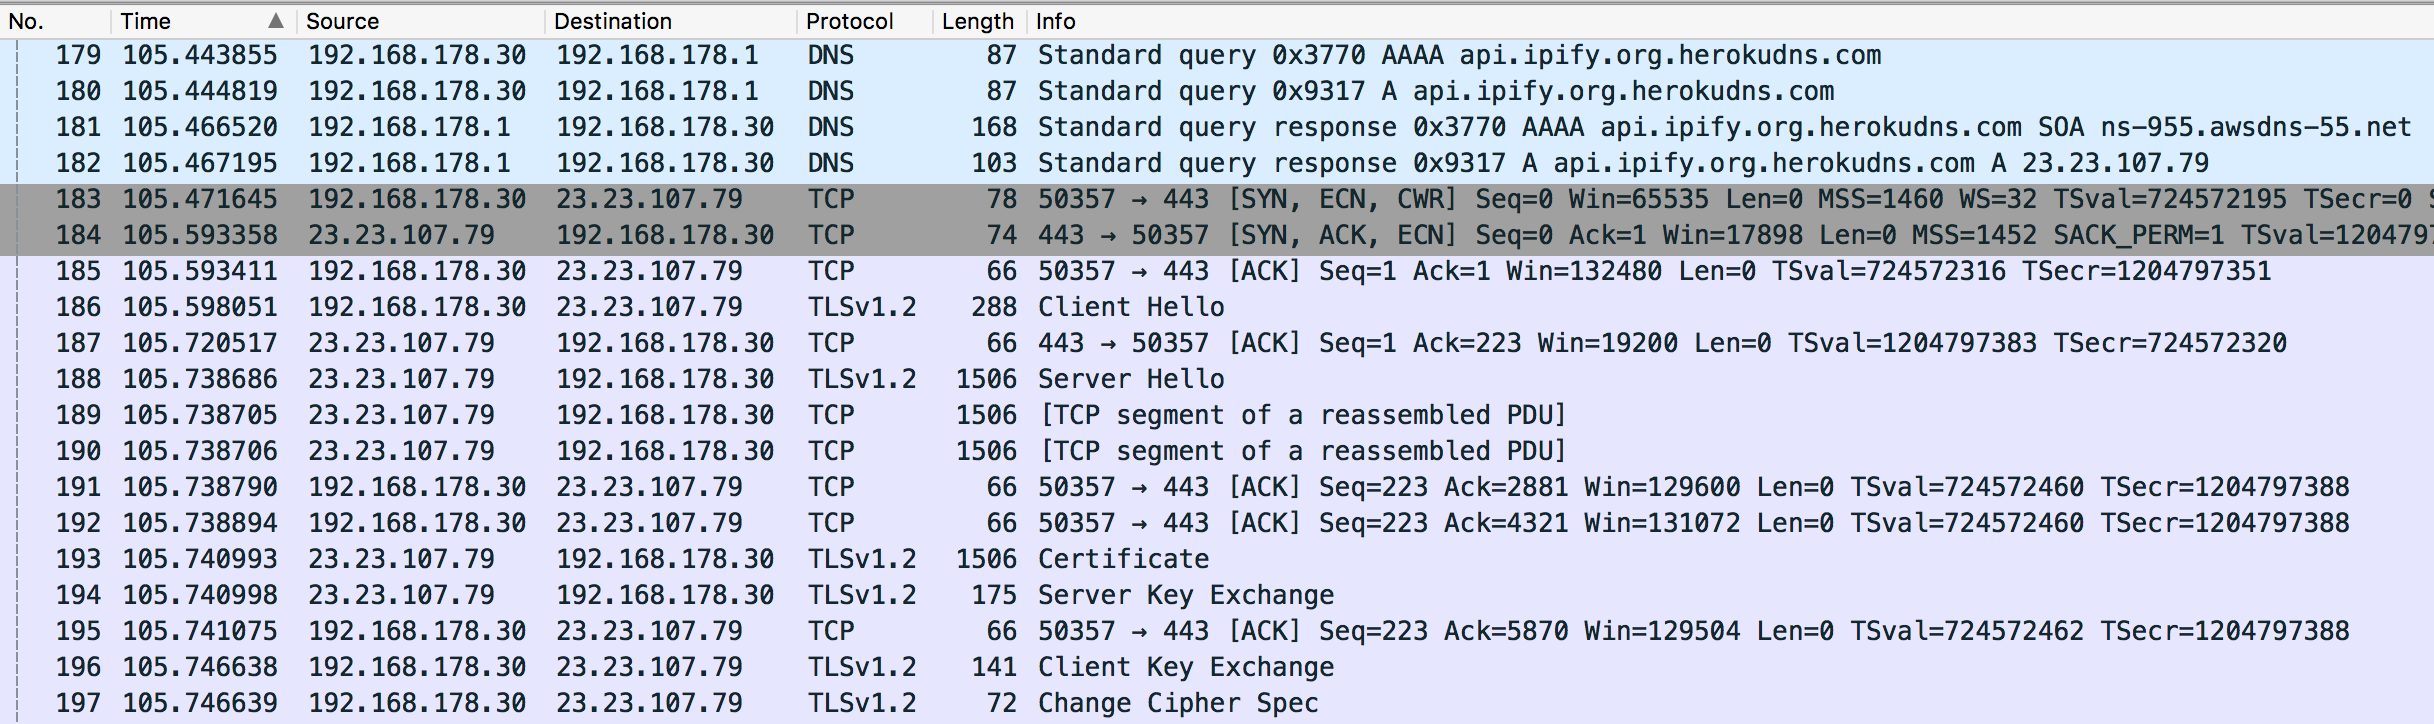
\includegraphics[width=\textwidth]{bilder/pentest_mobile_anwendungen/weiterentw_mobsf/wireshark_simulator.png}
	\caption{Verbindung zu \url{https://api.ipify.org} aus dem iOS-Simulator}
	\label{fig:WeitMobSFiOSWireshark}
\end{figure}

Aufgrund der strengen Vorkonfiguration bezüglich der Transport-Sicherung (siehe Abschnitt \ref{ref:inseccon}), ist mit mehr TLS-Verkehr als bei gewöhnlichen Anwendungen zu rechnen. Umso wichtiger ist es, diese unterbrechen und den Inhalt entschlüsseln zu können. Ein passendes Tool hierfür ist \textit{MITMProxy}, welches als lokaler Proxy-Server alle TLS-Verbindungen unterbricht. Zum Client hin wird ein selbst generiertes Zertifikat angeboten, während zum Webserver eine valide TLS-Verbindung aufgebaut wird. Dies hat natürlich den Nachteil, dass am emulierten Gerät dem selbst generierten Zertifikat vertraut werden muss. Auch zu prüfen bleiben die Möglichkeiten zur Einstellung des Proxy-Servers auf dem emulierten Gerät.\\

Zuerst wurde die Möglichkeit geprüft, das Zertifikat auf emulierten Geräten in den Trust-Store aufzunehmen. Da eine händische Aufnahme weder möglich, noch für die Automatisierung vorteilhaft wäre, sollte ein passendes Tool genutzt werden. \textit{ADVTOOLS}\footnote{\url{https://github.com/ADVTOOLS/ADVTrustStore}} ermöglicht es, eine beliebige \textit{CA} in den Trust-Store der emulierten Geräte aufzunehmen, und bietet damit die passende Funktionalität.\\

Als nächstes ist die Konfiguration von Proxy-Servern auf den emulierten Geräte zu realisieren. Auch dies ist leider nicht direkt über den Simulator realisierbar, jedoch nutzt der Simulator den Proxy-Server des\textit{ Mac OS X}-Host-Systems. Dieser kann über die System-Einstellungen konfiguriert werden (siehe Grafik \ref{fig:WeitMobSFiOSProxySettings}).\\

\begin{figure}[htbp]
	\centering
	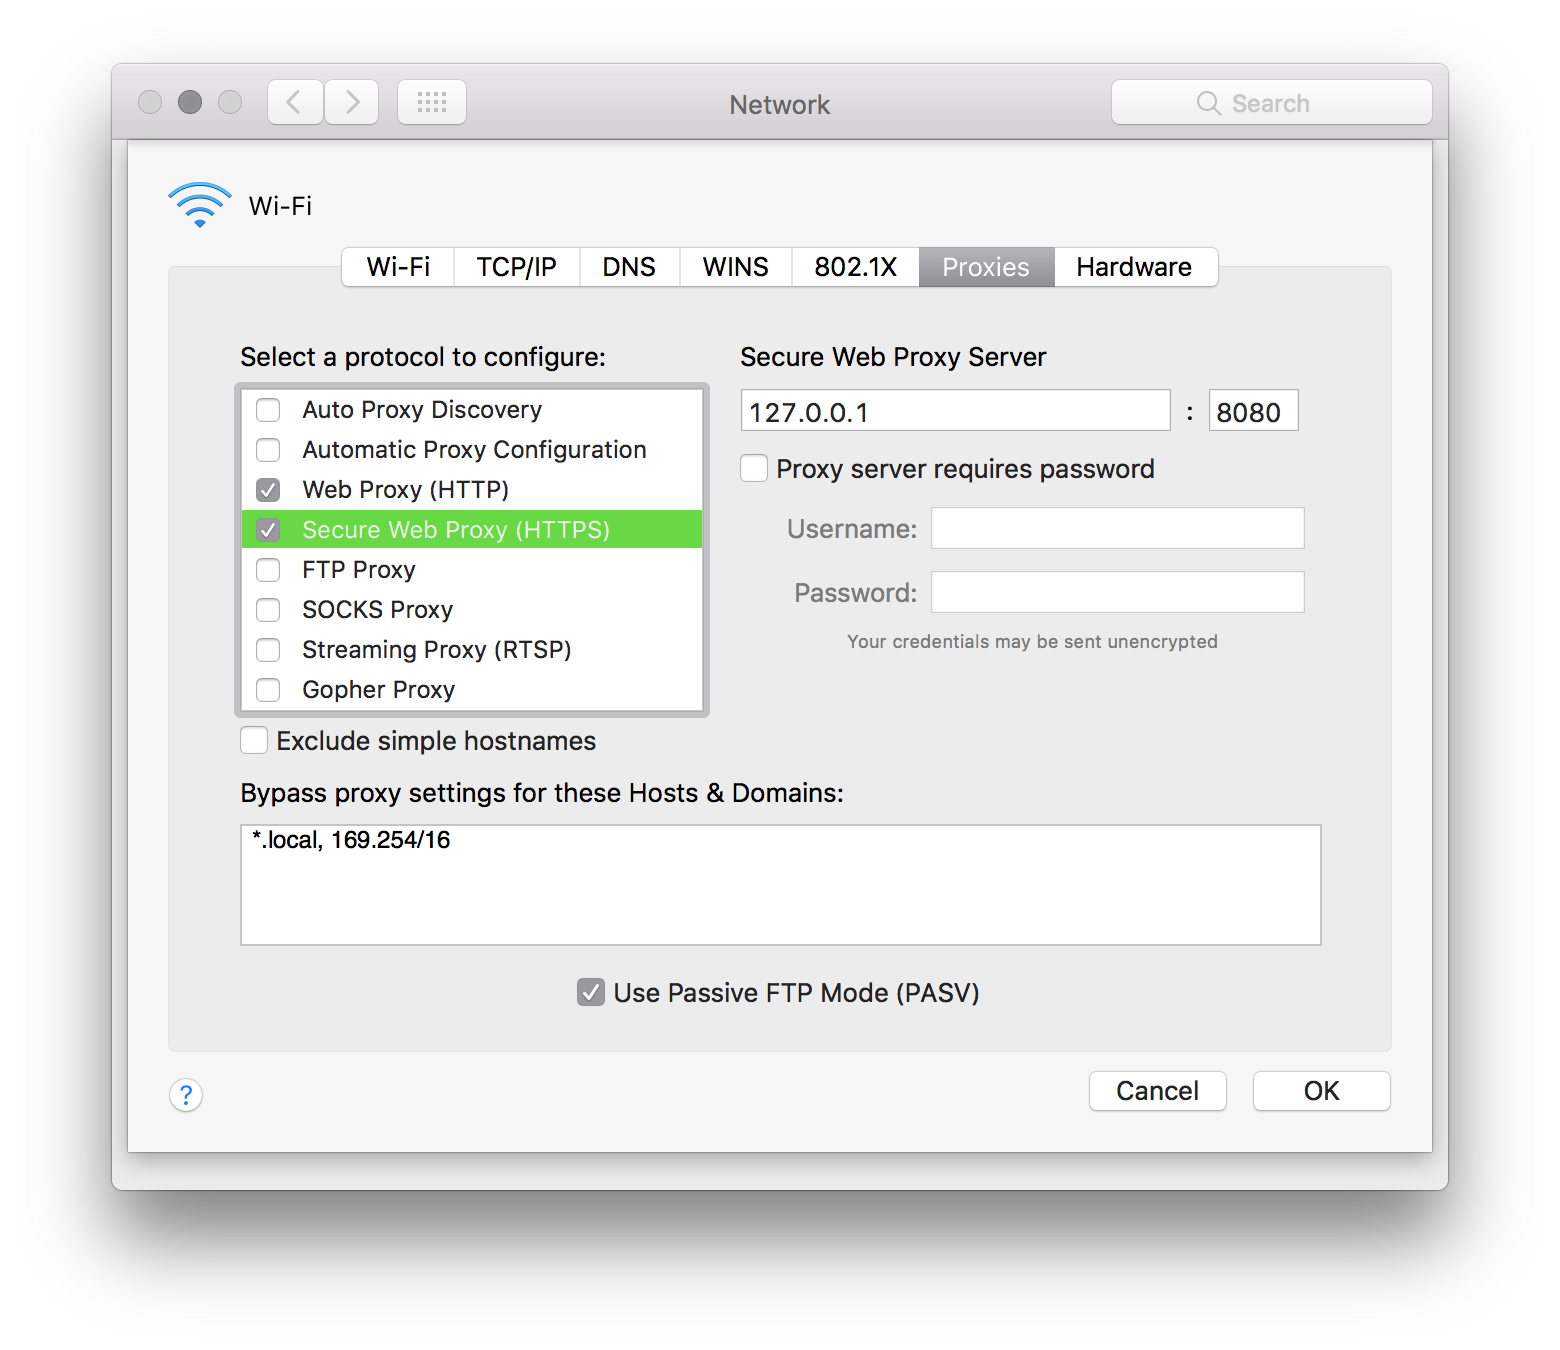
\includegraphics[width=\textwidth]{bilder/pentest_mobile_anwendungen/weiterentw_mobsf/proxy_settings.png}
	\caption{Einstellung des Proxy-Servers unter \textit{Mac OS X}}
	\label{fig:WeitMobSFiOSProxySettings}
\end{figure}

Somit ist nun eine TLS-Unterbrechung über \textit{MITMProxy} denkbar. \textit{MITMProxy} bietet eine \textit{NCurses}-Oberfläche an, um den durchlaufenden Netzwerkverkehr zu analysieren. Diese ist in Grafik \ref{fig:WeitMobSFiOSMITMProxUI} dargestellt.\\

\begin{figure}[htbp]
	\centering
	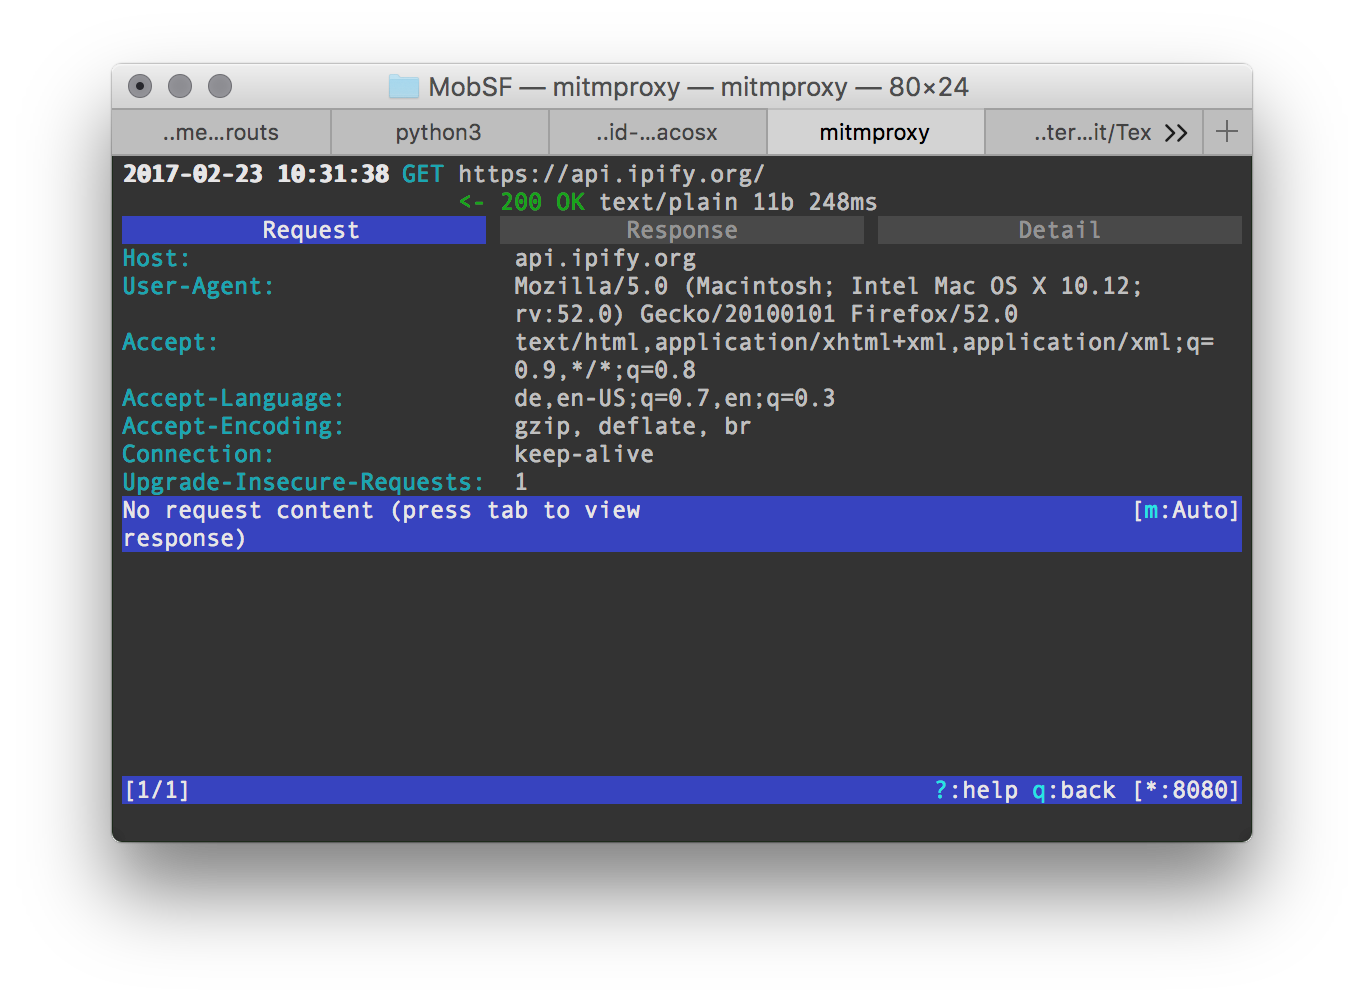
\includegraphics[width=\textwidth]{bilder/pentest_mobile_anwendungen/weiterentw_mobsf/mitmproxy_ncurses.png}
	\caption{Oberfläche von \textit{MITMProxy}}
	\label{fig:WeitMobSFiOSMITMProxUI}
\end{figure}

Diese Oberfläche ist jedoch für eine automatisierte Auswertung ungeeignet. Als zusätzliches Feature bietet \textit{MITMProxy} seine Funktionalität auch als Python-Modul an. Über diese wurde ein Server implementiert, welcher den Netzwerkverkehr aufzeichnet und in einem geeigneten Format ablegt. Der Server ist im Anhang unter \ref{ap:mitmserver} dargestellt.\\

Insoweit ist eine dynamische Analyse möglich. Der entsprechende Code, um alle Schritte zusammen zu führen, ist ebenfalls im Anhang unter \ref{ap:simcontrol} zu finden. Da jedoch, wie in \ref{ref:VergAktSitiOSArch} beschrieben, nur entsprechend kompilierte Apps oder solche, für welche der Sourcecode zur Verfügung steht, getestet werden können, ist der Use-Case für \textit{MobSF} relativ gering. Daher wird der Sourcecode zwar veröffentlicht, jedoch nicht in \textit{MobSF} integriert.\\

Im Laufe des Jahres soll eine Implementierung der dynamischen Analyse auf Basis eines physikalischen Geräts mit Jailbreak erfolgen. Dies ist jedoch nicht mehr Teil dieser Arbeit.

%http://eightbit.io/post/64319534191/how-to-set-up-an-ios-pen-testing-environment

%remote anzeige
%git://git.saurik.com/cydia.git
%http://kanaka.github.io/noVNC/ als front interface
%http://sharedinstance.net/2013/10/running-tweaks-in-simulator/ vnc server auf Iphone installieren, z.B. 
%TODO: Installation VNC-Server auf Simulator testen <-- Kein Chance
%TODO: VNC in Web-Oberfläche testen
		
	\section{Laboraufbau}
	\section{Entwicklung der Umgebung}
		\subsection{Aufbau}
		\subsection{Schnittstellen}
		\subsection{RPC-Service}
Um eine Kommunikation zwischen den verschiedenen Virtuellen Maschienen zu ermöglichen, wurde ein minimaler RPC-Server in Python 3.5 entwickelt. Verwendet wurden hierzu die Bibliotheken \textit{Flask} und \textit{Requests}.

\subsubsection{Flask}\label{ref:flask}
Flask ist ein schneller, minimaler Webserver. Mit nur sehr wenig Code es möglich, eine Schnittstelle bereit zu stellen. Ein Code mit zwei akzeptierenden Funktionen, basierend auf der Schnellstart-Anleitung\footnote{\url{http://flask.pocoo.org/docs/0.10/quickstart/}}, ist in Abbildung \ref{ref:rpc_client.py} dargestellt.
\begin{figure}
\begin{lstlisting}
from flask import Flask
app = Flask(__name__)

@app.route('/')
def hello_world():
	print("Execute command!")
    return 'Hello World!'
    
@app.route('/second_command/')
def not_hello_world():
	print("Execute second command!")
    return 'Goodbye World!'

if __name__ == '__main__':
    app.run()
\end{lstlisting}
\label{ref:rpc_client.py}
\caption{rpc\_client.py}
\end{figure}

Es wird eine minimale Anwendung erstellt, welche auf dem Pfad "\url{/}" lokal das print-Statement ausführt und den Text 'Hello World!' zurück gibt. 
Wir die Anwendung unter dem Pfad "\url{/second_command/}" angesprochen, wird ein anderes print-Statement ausgeführt und ein anderer Wert zurück gegeben. Auf diese Weise können schnell API-Funktionen auf verschiedene Pfade gelegt und angesprochen werden.

\subsubsection{Requests}
Requests ist eine Python-Bibliothek, welche einfache Anfragen (sogenannte Requests, daher der Name) an Web-Server ermöglicht. So ist es über ein kurzes Code-Snippet, dargestellt in Abbildung \ref{ref:rpc_server.py}, möglich die unter \ref{ref:rpc_client.py} aufgezeigt Schnittstelle anzusprechen.

\begin{figure}
\begin{lstlisting}
import requests

r = requests.get('http://localhost:5000')
print(r.text)

r = requests.get('http://localhost:5000/second_command/')
print(r.text)
\end{lstlisting}
\label{ref:rpc_server.py}
\caption{rpc\_server.py}
\end{figure}

Wird zuerst der Code \ref{ref:rpc_client.py} und anschließend der Code \ref{ref:rpc_server.py} ausgeführt, wird auf Server-Seite folgende Ausgabe erzeugt:
\begin{lstlisting}
 $ python3 rpc_server.py
Hello World!
Goodbye World!
\end{lstlisting}
Auf der Client-Seite erfolgt folgende Ausgabe:
\begin{lstlisting}
 $ python3 rpc_client.py
 * Running on http://127.0.0.1:5000/
Execute command!
127.0.0.1 - - [18/May/2016 19:10:56] "GET / HTTP/1.1" 200 -
Execute second command!
127.0.0.1 - - [18/May/2016 19:10:56] "GET /second_command/ HTTP/1.1" 200 -
\end{lstlisting}

Aufgrund dieser Basis wurde das RPC-Tool implementiert.


		\subsection{Technisches Detail 1}
		\subsection{Technisches Detail 2}
	\section{Abgleich mit Anforderungen}